\section{Casi d'uso}
I casi d'uso seguenti emergono da un'attenta analisi degli \textit{Analisti} del gruppo \GroupName{} rivolta al capitolato e da un'approfondita discussione con il proponente Proponente{}. Gran parte dei casi d'uso sono stati dedotti grazie all'esperienza derivata dall'utilizzo di glossario{ActiveAdmin}, un progetto analogo a \ProjectName{} basato su glossario{Ruby on Rails}.\
Ogni caso d'uso è identificato univocamente e in modo gerarchico tramite una codifica nella forma:

\begin{center}

\textit{UC[codice dell'ambito][codice univoco del padre],[codice progressivo del figlio]}

\end{center} 

dove il \textbf{codice dell'ambito} può assumere i seguenti valori:

\begin{itemize}

  \item \textbf{U} - ambito utente, che comprende sia l'utente normale che l'\textit{admin} di una applicazione generata da \ProjectName{};
  \item \textbf{S} - ambito sviluppatore.

\end{itemize}

\subsection{Ambito Utente}
\subsubsection{UCS3.3.1.9 - Definizione azioni personalizzate}
    
    \begin{figure}[H]
      %\includegraphics[width=12cm]{UML/UCS3.3.1.9 - Definizione azioni personalizzate.png}
      \caption{UCU - Operazioni ad alto livello} 
    \end{figure}
      
    %Tabella 
      \begin{table}[h]
      \begin{longtabu}{  c | X  }
            
      \hline
      \multicolumn{2}{ | c | }{ \cellcolor[gray]{0.9} \textbf{UCS3.3.1.9 - Definizione azioni personalizzate}} \\ 
      \hline
      
       & \\
      
      \textbf{Attori Primari} & Sviluppatore \\ 
          \textbf{Attori Secondari} &   \\
          \textbf{Scopo e Descrizione} & Lo sviluppatore all'interno del file di configurazione della Collection definisce delle azioni personalizzate che potranno essere eseguite dall'applicazione. Deve essere possibile specificare dei permessi per l'esecuzione di ciascuna azione personalizzata, in caso venga omessa chiunque potrà eseguirla. \\ 
          
          \textbf{Precondizioni}  & Il Framework MaaP è funzionante e la Collection è registrata.\\ 
          
          \textbf{Postcondizioni} & Il Framework MaaP ha apportato le modifiche alla configurazione della Collection. \\
          
          \textbf{Flusso Principale} &  \\
           \textbf{Scenari Alternativi} &  \\
      \end{longtabu}
      \end{table}
\subsubsection{UCS3.3.2 - Personalizzazione show page}
    
    \begin{figure}[H]
      %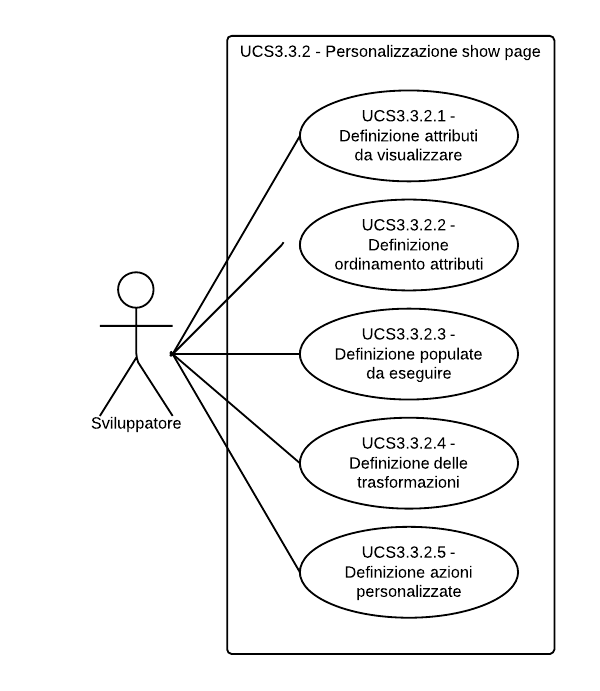
\includegraphics[width=12cm]{UML/UCS3.3.2 - Personalizzazione show page.png}
      \caption{UCU - Operazioni ad alto livello} 
    \end{figure}
      
    %Tabella 
      \begin{table}[h]
      \begin{longtabu}{  c | X  }
            
      \hline
      \multicolumn{2}{ | c | }{ \cellcolor[gray]{0.9} \textbf{UCS3.3.2 - Personalizzazione show page}} \\ 
      \hline
      
       & \\
      
      \textbf{Attori Primari} & Sviluppatore \\ 
          \textbf{Attori Secondari} &   \\
          \textbf{Scopo e Descrizione} & Lo sviluppatore personalizza la show page della Collection selezionata. \\ 
          
          \textbf{Precondizioni}  & Il Framework MaaP è funzionante e la Collection da configurare è stata registrata.\\ 
          
          \textbf{Postcondizioni} & Il Framework MaaP ha configurato correttamente la show page della Collection. \\
          
          \textbf{Flusso Principale} & 1. Lo sviluppatore definisce gli attributi da visualizzare nella show page (UCS3.3.2.1);
2. Lo sviluppatore definisce l'ordinamento degli attributi nella show page (UCS3.3.2.2);
3. Lo sviluppatore definisce attributi che contengono attributi innestati o array di attributi (UCS3.3.2.3);
4. Lo sviluppatore definisce delle trasformazioni sugli attributi (UCS3.3.2.4);
5. Lo sviluppatore definisce delle azioni personalizzate da eseguire all'interno della show page (UCS3.3.2.5). \\
           \textbf{Scenari Alternativi} &  \\
      \end{longtabu}
      \end{table}
\subsubsection{UCS2.1 - Configurazione database credenziali}
    
    \begin{figure}[H]
      %\includegraphics[width=12cm]{UML/UCS2.1 - Configurazione database credenziali.png}
      \caption{UCU - Operazioni ad alto livello} 
    \end{figure}
      
    %Tabella 
      \begin{table}[h]
      \begin{longtabu}{  c | X  }
            
      \hline
      \multicolumn{2}{ | c | }{ \cellcolor[gray]{0.9} \textbf{UCS2.1 - Configurazione database credenziali}} \\ 
      \hline
      
       & \\
      
      \textbf{Attori Primari} & Sviluppatore \\ 
          \textbf{Attori Secondari} &   \\
          \textbf{Scopo e Descrizione} & Lo sviluppatore può configurare il database che conterrà le credenziali degli utenti i quali utilizzeranno l'applicazione generata dal Framework. \\ 
          
          \textbf{Precondizioni}  & Il Framework permette la configurazione del database credenziali.\\ 
          
          \textbf{Postcondizioni} & Il Framework Maap ha configurato il database delle credenziali secondo le informazioni acquisite dallo sviluppatore. \\
          
          \textbf{Flusso Principale} &  \\
           \textbf{Scenari Alternativi} &  \\
      \end{longtabu}
      \end{table}
\subsubsection{UCS2 - Configurazione database}
    
    \begin{figure}[H]
      %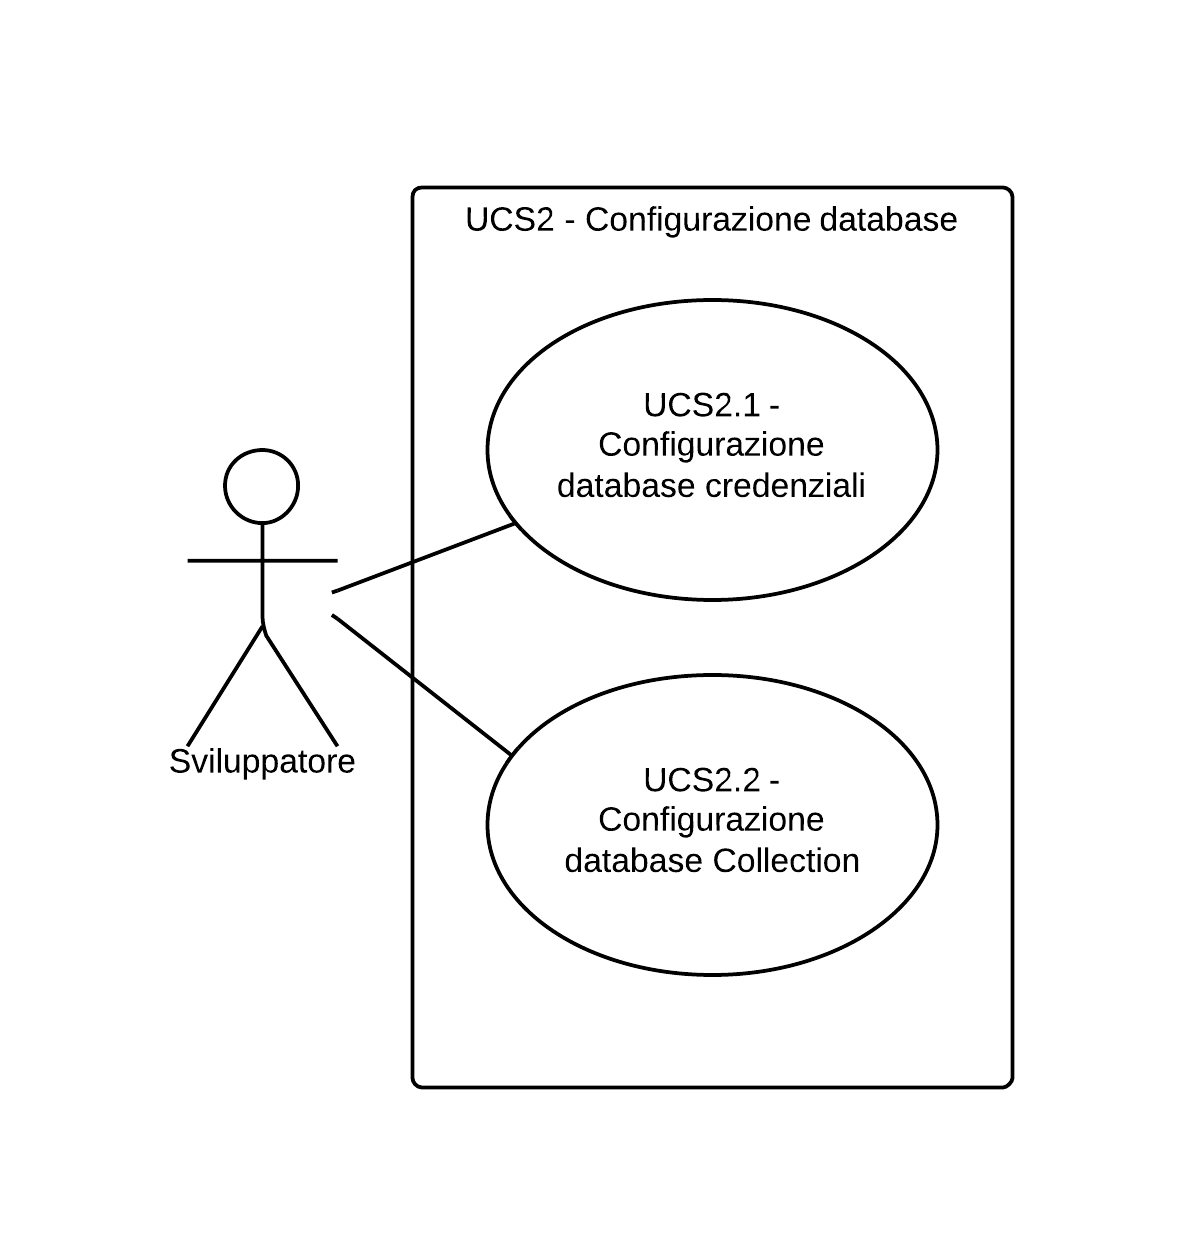
\includegraphics[width=12cm]{UML/UCS2 - Configurazione database.png}
      \caption{UCU - Operazioni ad alto livello} 
    \end{figure}
      
    %Tabella 
      \begin{table}[h]
      \begin{longtabu}{  c | X  }
            
      \hline
      \multicolumn{2}{ | c | }{ \cellcolor[gray]{0.9} \textbf{UCS2 - Configurazione database}} \\ 
      \hline
      
       & \\
      
      \textbf{Attori Primari} & Sviluppatore \\ 
          \textbf{Attori Secondari} &   \\
          \textbf{Scopo e Descrizione} & Lo sviluppatore può configurare i due database che compongono il sistema Maap, ovvero il database delle credenziali utenti e il database contenente le collection. \\ 
          
          \textbf{Precondizioni}  & Framework è funzionante, il progetto è stato creato e lo sviluppatore desidera configurare i database.\\ 
          
          \textbf{Postcondizioni} & Il Framework ha ottenuto le informazioni necessarie ed ha configurato il database delle credenziali e il database delle collection. \\
          
          \textbf{Flusso Principale} &  \\
           \textbf{Scenari Alternativi} &  \\
      \end{longtabu}
      \end{table}
\subsubsection{UCS3.3.1.6 - Definizione populate da eseguire}
    
    \begin{figure}[H]
      %\includegraphics[width=12cm]{UML/UCS3.3.1.6 - Definizione populate da eseguire.png}
      \caption{UCU - Operazioni ad alto livello} 
    \end{figure}
      
    %Tabella 
      \begin{table}[h]
      \begin{longtabu}{  c | X  }
            
      \hline
      \multicolumn{2}{ | c | }{ \cellcolor[gray]{0.9} \textbf{UCS3.3.1.6 - Definizione populate da eseguire}} \\ 
      \hline
      
       & \\
      
      \textbf{Attori Primari} & Sviluppatore \\ 
          \textbf{Attori Secondari} &   \\
          \textbf{Scopo e Descrizione} & Lo sviluppatore all'interno del file di configurazione della Collection specifica attributi che contengono attributi innestati o un array di Document tramite la funzione populate. \\ 
          
          \textbf{Precondizioni}  & Il Framework MaaP è funzionante e la Collection è registrata.\\ 
          
          \textbf{Postcondizioni} & Il Framework MaaP ha apportato le modifiche alla configurazione della Collection. \\
          
          \textbf{Flusso Principale} &  \\
           \textbf{Scenari Alternativi} &  \\
      \end{longtabu}
      \end{table}
\subsubsection{UCS3.3.1.7 - Personalizzazione filtri}
    
    \begin{figure}[H]
      %\includegraphics[width=12cm]{UML/UCS3.3.1.7 - Personalizzazione filtri.png}
      \caption{UCU - Operazioni ad alto livello} 
    \end{figure}
      
    %Tabella 
      \begin{table}[h]
      \begin{longtabu}{  c | X  }
            
      \hline
      \multicolumn{2}{ | c | }{ \cellcolor[gray]{0.9} \textbf{UCS3.3.1.7 - Personalizzazione filtri}} \\ 
      \hline
      
       & \\
      
      \textbf{Attori Primari} & Sviluppatore \\ 
          \textbf{Attori Secondari} &   \\
          \textbf{Scopo e Descrizione} & Lo sviluppatore all'interno del file di configurazione della Collection specifica quali filtri inserire nella index page. \\ 
          
          \textbf{Precondizioni}  & Il Framework MaaP è funzionante e la Collection è registrata.\\ 
          
          \textbf{Postcondizioni} & Il Framework MaaP ha apportato le modifiche alla configurazione della Collection. \\
          
          \textbf{Flusso Principale} &  \\
           \textbf{Scenari Alternativi} &  \\
      \end{longtabu}
      \end{table}
\subsubsection{UCS3.3.1.8 - Definizione delle trasformazioni}
    
    \begin{figure}[H]
      %\includegraphics[width=12cm]{UML/UCS3.3.1.8 - Definizione delle trasformazioni.png}
      \caption{UCU - Operazioni ad alto livello} 
    \end{figure}
      
    %Tabella 
      \begin{table}[h]
      \begin{longtabu}{  c | X  }
            
      \hline
      \multicolumn{2}{ | c | }{ \cellcolor[gray]{0.9} \textbf{UCS3.3.1.8 - Definizione delle trasformazioni}} \\ 
      \hline
      
       & \\
      
      \textbf{Attori Primari} & Sviluppatore \\ 
          \textbf{Attori Secondari} &   \\
          \textbf{Scopo e Descrizione} & Lo sviluppatore all'interno del file di configurazione della Collection specifica delle trasformazioni sui valori degli attributi che visualizzeranno l'attributo in base all'output della funzione di trasformazione. \\ 
          
          \textbf{Precondizioni}  & Il Framework MaaP è funzionante e la Collection è registrata.\\ 
          
          \textbf{Postcondizioni} & Il Framework MaaP ha apportato le modifiche alla configurazione della Collection. \\
          
          \textbf{Flusso Principale} &  \\
           \textbf{Scenari Alternativi} &  \\
      \end{longtabu}
      \end{table}
\subsubsection{UCS3.3.2.1 - Definizione attributi da visualizzare}
    
    \begin{figure}[H]
      %\includegraphics[width=12cm]{UML/UCS3.3.2.1 - Definizione attributi da visualizzare.png}
      \caption{UCU - Operazioni ad alto livello} 
    \end{figure}
      
    %Tabella 
      \begin{table}[h]
      \begin{longtabu}{  c | X  }
            
      \hline
      \multicolumn{2}{ | c | }{ \cellcolor[gray]{0.9} \textbf{UCS3.3.2.1 - Definizione attributi da visualizzare}} \\ 
      \hline
      
       & \\
      
      \textbf{Attori Primari} & Sviluppatore \\ 
          \textbf{Attori Secondari} &   \\
          \textbf{Scopo e Descrizione} & Lo sviluppatore all'interno del file di configurazione della Collection specifica quali attributi visualizzare nella show page. \\ 
          
          \textbf{Precondizioni}  & Il Framework MaaP è funzionante e la Collection è registrata.\\ 
          
          \textbf{Postcondizioni} & Il Framework MaaP ha apportato le modifiche alla configurazione della Collection. \\
          
          \textbf{Flusso Principale} &  \\
           \textbf{Scenari Alternativi} &  \\
      \end{longtabu}
      \end{table}
\subsubsection{UCS3.3.2.2 - Definizione ordinamento attributi}
    
    \begin{figure}[H]
      %\includegraphics[width=12cm]{UML/UCS3.3.2.2 - Definizione ordinamento attributi.png}
      \caption{UCU - Operazioni ad alto livello} 
    \end{figure}
      
    %Tabella 
      \begin{table}[h]
      \begin{longtabu}{  c | X  }
            
      \hline
      \multicolumn{2}{ | c | }{ \cellcolor[gray]{0.9} \textbf{UCS3.3.2.2 - Definizione ordinamento attributi}} \\ 
      \hline
      
       & \\
      
      \textbf{Attori Primari} & Sviluppatore \\ 
          \textbf{Attori Secondari} &   \\
          \textbf{Scopo e Descrizione} & Lo sviluppatore all'interno del file di configurazione della Collection specifica l'ordinamento degli attributi da visualizzare nella show page. \\ 
          
          \textbf{Precondizioni}  & Il Framework MaaP è funzionante e la Collection è registrata.\\ 
          
          \textbf{Postcondizioni} & Il Framework MaaP ha apportato le modifiche alla configurazione della Collection. \\
          
          \textbf{Flusso Principale} &  \\
           \textbf{Scenari Alternativi} &  \\
      \end{longtabu}
      \end{table}
\subsubsection{UCS3.3.2.3 - Definizione populate da eseguire}
    
    \begin{figure}[H]
      %\includegraphics[width=12cm]{UML/UCS3.3.2.3 - Definizione populate da eseguire.png}
      \caption{UCU - Operazioni ad alto livello} 
    \end{figure}
      
    %Tabella 
      \begin{table}[h]
      \begin{longtabu}{  c | X  }
            
      \hline
      \multicolumn{2}{ | c | }{ \cellcolor[gray]{0.9} \textbf{UCS3.3.2.3 - Definizione populate da eseguire}} \\ 
      \hline
      
       & \\
      
      \textbf{Attori Primari} & Sviluppatore \\ 
          \textbf{Attori Secondari} &   \\
          \textbf{Scopo e Descrizione} & Lo sviluppatore all'interno del file di configurazione della Collection specifica attributi che contengono attributi innestati o un array di Document tramite la funzione populate. \\ 
          
          \textbf{Precondizioni}  & Il Framework MaaP è funzionante e la Collection è registrata.\\ 
          
          \textbf{Postcondizioni} & Il Framework MaaP ha apportato le modifiche alla configurazione della Collection. \\
          
          \textbf{Flusso Principale} &  \\
           \textbf{Scenari Alternativi} &  \\
      \end{longtabu}
      \end{table}
\subsubsection{UCS3.3.2.4 - Definizione delle trasformazioni}
    
    \begin{figure}[H]
      %\includegraphics[width=12cm]{UML/UCS3.3.2.4 - Definizione delle trasformazioni.png}
      \caption{UCU - Operazioni ad alto livello} 
    \end{figure}
      
    %Tabella 
      \begin{table}[h]
      \begin{longtabu}{  c | X  }
            
      \hline
      \multicolumn{2}{ | c | }{ \cellcolor[gray]{0.9} \textbf{UCS3.3.2.4 - Definizione delle trasformazioni}} \\ 
      \hline
      
       & \\
      
      \textbf{Attori Primari} & Sviluppatore \\ 
          \textbf{Attori Secondari} &   \\
          \textbf{Scopo e Descrizione} & Lo sviluppatore all'interno del file di configurazione della Collection specifica delle trasformazioni sui valori degli attributi che visualizzeranno l'attributo in base all'output della funzione di trasformazione. \\ 
          
          \textbf{Precondizioni}  & Il Framework MaaP è funzionante e la Collection è registrata.\\ 
          
          \textbf{Postcondizioni} & Il Framework MaaP ha apportato le modifiche alla configurazione della Collection. \\
          
          \textbf{Flusso Principale} &  \\
           \textbf{Scenari Alternativi} &  \\
      \end{longtabu}
      \end{table}
\subsubsection{UCS3.3.2.5 - Definizione azioni personalizzate}
    
    \begin{figure}[H]
      %\includegraphics[width=12cm]{UML/UCS3.3.2.5 - Definizione azioni personalizzate.png}
      \caption{UCU - Operazioni ad alto livello} 
    \end{figure}
      
    %Tabella 
      \begin{table}[h]
      \begin{longtabu}{  c | X  }
            
      \hline
      \multicolumn{2}{ | c | }{ \cellcolor[gray]{0.9} \textbf{UCS3.3.2.5 - Definizione azioni personalizzate}} \\ 
      \hline
      
       & \\
      
      \textbf{Attori Primari} & Sviluppatore \\ 
          \textbf{Attori Secondari} &   \\
          \textbf{Scopo e Descrizione} & Lo sviluppatore all'interno del file di configurazione della Collection definisce delle azioni personalizzate che potranno essere eseguite dalla show page. Deve essere possibile specificare dei permessi per l'esecuzione di ciascuna azione personalizzata, in caso venga omessa chiunque potrà eseguirla. \\ 
          
          \textbf{Precondizioni}  & Il Framework MaaP è funzionante e la Collection è registrata.\\ 
          
          \textbf{Postcondizioni} & Il Framework MaaP ha apportato le modifiche alla configurazione della Collection. \\
          
          \textbf{Flusso Principale} &  \\
           \textbf{Scenari Alternativi} &  \\
      \end{longtabu}
      \end{table}
\subsubsection{UCU3 - Logout}
    
    \begin{figure}[H]
      %\includegraphics[width=12cm]{UML/UCU3 - Logout.png}
      \caption{UCU - Operazioni ad alto livello} 
    \end{figure}
      
    %Tabella 
      \begin{table}[h]
      \begin{longtabu}{  c | X  }
            
      \hline
      \multicolumn{2}{ | c | }{ \cellcolor[gray]{0.9} \textbf{UCU3 - Logout}} \\ 
      \hline
      
       & \\
      
      \textbf{Attori Primari} & Utente autenticato, Admin \\ 
          \textbf{Attori Secondari} &   \\
          \textbf{Scopo e Descrizione} & L'utente autenticato può eseguire il logout dall'applicazione. \\ 
          
          \textbf{Precondizioni}  & L'applicazione mette a disposizione all'utente la possibilità di logout.\\ 
          
          \textbf{Postcondizioni} & L'applicazione ha eseguito il logout richiesto dall'utente. \\
          
          \textbf{Flusso Principale} &  \\
           \textbf{Scenari Alternativi} &  \\
      \end{longtabu}
      \end{table}
\subsubsection{UCU10 - Modifica profilo}
    
    \begin{figure}[H]
      %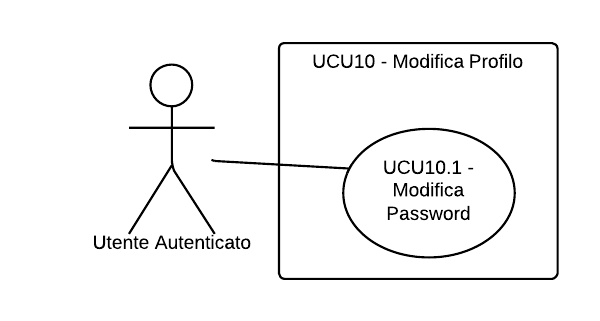
\includegraphics[width=12cm]{UML/UCU10 - Modifica profilo.png}
      \caption{UCU - Operazioni ad alto livello} 
    \end{figure}
      
    %Tabella 
      \begin{table}[h]
      \begin{longtabu}{  c | X  }
            
      \hline
      \multicolumn{2}{ | c | }{ \cellcolor[gray]{0.9} \textbf{UCU10 - Modifica profilo}} \\ 
      \hline
      
       & \\
      
      \textbf{Attori Primari} & Utente autenticato \\ 
          \textbf{Attori Secondari} &   \\
          \textbf{Scopo e Descrizione} & L'utente autenticato ha a disposizione una pagina in cui poter modificare il proprio profilo, modificando email e/o password. \\ 
          
          \textbf{Precondizioni}  & L'utente si trova all'interno della pagina di modifica del proprio profilo.\\ 
          
          \textbf{Postcondizioni} & L'utente ha modificato il proprio profilo e il database è stato aggiornato. \\
          
          \textbf{Flusso Principale} & 1. L'utente autenticato modifica la propria email (UCU10.1);
2. L'utente autenticato modifica la propria password (UCU10.2); \\
           \textbf{Scenari Alternativi} &  \\
      \end{longtabu}
      \end{table}
\subsubsection{UCU10.1 - Modifica email}
    
    \begin{figure}[H]
      %\includegraphics[width=12cm]{UML/UCU10.1 - Modifica email.png}
      \caption{UCU - Operazioni ad alto livello} 
    \end{figure}
      
    %Tabella 
      \begin{table}[h]
      \begin{longtabu}{  c | X  }
            
      \hline
      \multicolumn{2}{ | c | }{ \cellcolor[gray]{0.9} \textbf{UCU10.1 - Modifica email}} \\ 
      \hline
      
       & \\
      
      \textbf{Attori Primari} & Utente autenticato \\ 
          \textbf{Attori Secondari} &   \\
          \textbf{Scopo e Descrizione} & L'utente autenticato inserisce la nuova email in un apposito campo di testo. \\ 
          
          \textbf{Precondizioni}  & L'utente autenticato si trova all'interno della pagina di modifica del proprio profilo.\\ 
          
          \textbf{Postcondizioni} & L'utente ha inserito la nuova email all'interno dell'apposito campo. \\
          
          \textbf{Flusso Principale} &  \\
           \textbf{Scenari Alternativi} &  \\
      \end{longtabu}
      \end{table}
\subsubsection{UCU10.2 - Modifica password}
    
    \begin{figure}[H]
      %\includegraphics[width=12cm]{UML/UCU10.2 - Modifica password.png}
      \caption{UCU - Operazioni ad alto livello} 
    \end{figure}
      
    %Tabella 
      \begin{table}[h]
      \begin{longtabu}{  c | X  }
            
      \hline
      \multicolumn{2}{ | c | }{ \cellcolor[gray]{0.9} \textbf{UCU10.2 - Modifica password}} \\ 
      \hline
      
       & \\
      
      \textbf{Attori Primari} & Utente autenticato \\ 
          \textbf{Attori Secondari} &   \\
          \textbf{Scopo e Descrizione} & L'utente autenticato inserisce la nuova password in un apposito campo di testo. \\ 
          
          \textbf{Precondizioni}  & L'utente autenticato si trova all'interno della pagina di modifica del proprio profilo.\\ 
          
          \textbf{Postcondizioni} & L'utente ha inserito la nuova password all'interno dell'apposito campo. \\
          
          \textbf{Flusso Principale} &  \\
           \textbf{Scenari Alternativi} &  \\
      \end{longtabu}
      \end{table}
\subsubsection{UCU4 - Password Recovery}
    
    \begin{figure}[H]
      %\includegraphics[width=12cm]{UML/UCU4 - Password Recovery.png}
      \caption{UCU - Operazioni ad alto livello} 
    \end{figure}
      
    %Tabella 
      \begin{table}[h]
      \begin{longtabu}{  c | X  }
            
      \hline
      \multicolumn{2}{ | c | }{ \cellcolor[gray]{0.9} \textbf{UCU4 - Password Recovery}} \\ 
      \hline
      
       & \\
      
      \textbf{Attori Primari} & Utente non autenticato  \\ 
          \textbf{Attori Secondari} &   \\
          \textbf{Scopo e Descrizione} & L'utente intende recuperare la password d'accesso all'applicazione. \\ 
          
          \textbf{Precondizioni}  & L'applicazione predispone e mostra all'utente la possibilità di password recovery.\\ 
          
          \textbf{Postcondizioni} & L'applicazione ha effettuato le operazioni necessarie per la password recovery richiesta dall'utente. \\
          
          \textbf{Flusso Principale} &  \\
           \textbf{Scenari Alternativi} &  \\
      \end{longtabu}
      \end{table}
\subsubsection{UCU5 - Registrazione}
    
    \begin{figure}[H]
      %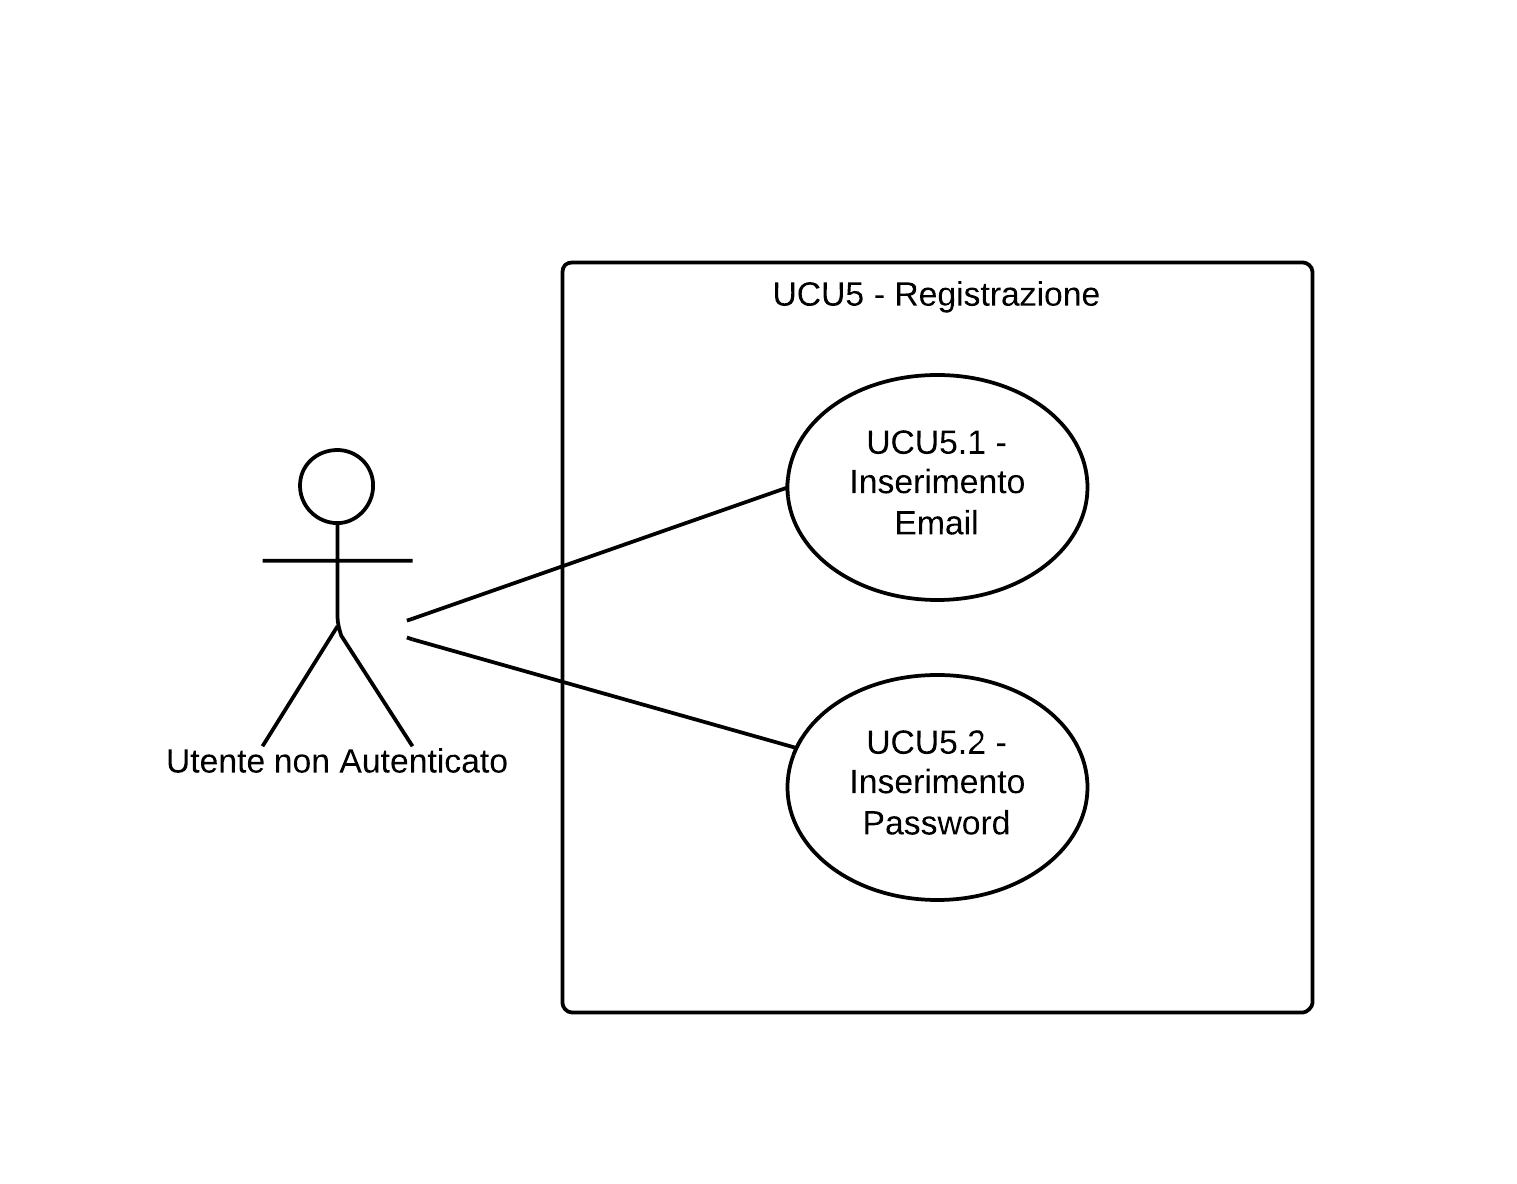
\includegraphics[width=12cm]{UML/UCU5 - Registrazione.png}
      \caption{UCU - Operazioni ad alto livello} 
    \end{figure}
      
    %Tabella 
      \begin{table}[h]
      \begin{longtabu}{  c | X  }
            
      \hline
      \multicolumn{2}{ | c | }{ \cellcolor[gray]{0.9} \textbf{UCU5 - Registrazione}} \\ 
      \hline
      
       & \\
      
      \textbf{Attori Primari} & Utente non autenticato  \\ 
          \textbf{Attori Secondari} &   \\
          \textbf{Scopo e Descrizione} & L'utente intende registrarsi all'applicazione e per farlo deve inserire negli appositi campi email e password. \\ 
          
          \textbf{Precondizioni}  & L'applicazione predispone la possibilità di registrazione.\\ 
          
          \textbf{Postcondizioni} & L'applicazione ha creato un nuovo account utente. \\
          
          \textbf{Flusso Principale} & 1. L'utente non autenticato inserisce l'email (UCU5.1);
2. L'utente non autenticato inserisce la password (UCU5.2). \\
           \textbf{Scenari Alternativi} & 1. L'utente non autenticato interrompe l'operazione di registrazione non creando un nuovo account. \\
      \end{longtabu}
      \end{table}
\subsubsection{UCU6 - Registrazione fallita}
    
    \begin{figure}[H]
      %\includegraphics[width=12cm]{UML/UCU6 - Registrazione fallita.png}
      \caption{UCU - Operazioni ad alto livello} 
    \end{figure}
      
    %Tabella 
      \begin{table}[h]
      \begin{longtabu}{  c | X  }
            
      \hline
      \multicolumn{2}{ | c | }{ \cellcolor[gray]{0.9} \textbf{UCU6 - Registrazione fallita}} \\ 
      \hline
      
       & \\
      
      \textbf{Attori Primari} & Utente non autenticato  \\ 
          \textbf{Attori Secondari} &   \\
          \textbf{Scopo e Descrizione} & L'utente visualizza un messaggio di errore dato dal fallimento del tentativo di registrazione effettuato. \\ 
          
          \textbf{Precondizioni}  & L'applicazione ha ricevuto i dati di registrazione inseriti dall'utente e tenta la creazione di un nuovo account.\\ 
          
          \textbf{Postcondizioni} & L'applicazione mostra un messaggio di errore per il fallimento del tentativo di registrazione richiesta dall'utente. \\
          
          \textbf{Flusso Principale} &  \\
           \textbf{Scenari Alternativi} &  \\
      \end{longtabu}
      \end{table}
\subsubsection{UCU11 - Pagina Admin}
    
    \begin{figure}[H]
      %\includegraphics[width=12cm]{UML/UCU11 - Pagina Admin.png}
      \caption{UCU - Operazioni ad alto livello} 
    \end{figure}
      
    %Tabella 
      \begin{table}[h]
      \begin{longtabu}{  c | X  }
            
      \hline
      \multicolumn{2}{ | c | }{ \cellcolor[gray]{0.9} \textbf{UCU11 - Pagina Admin}} \\ 
      \hline
      
       & \\
      
      \textbf{Attori Primari} & Admin \\ 
          \textbf{Attori Secondari} &   \\
          \textbf{Scopo e Descrizione} & L'admin entra nella sua pagina di amministrazione dalla quale visualizza una  Collection-index di tutti gli utenti registrati al sistema. \\ 
          
          \textbf{Precondizioni}  & Il sistema mostra all'admin la sua pagina di amministrazione\\ 
          
          \textbf{Postcondizioni} & Il sistema mette a disposizione dell'admin tutte le funzionalità di controllo previste. \\
          
          \textbf{Flusso Principale} & 1. L'admin può creare un nuovo utente (UCU11.1)
2. L'admin può visualizzare la Collection-show di un utente (UCU11.3) \\
           \textbf{Scenari Alternativi} & 1.1 - Fallisce l'inserimento di un nuovo utente (UCU11.2) \\
      \end{longtabu}
      \end{table}
\subsubsection{UCU8 - Apri Dashboard}
    
    \begin{figure}[H]
      %\includegraphics[width=12cm]{UML/UCU8 - Apri Dashboard.png}
      \caption{UCU - Operazioni ad alto livello} 
    \end{figure}
      
    %Tabella 
      \begin{table}[h]
      \begin{longtabu}{  c | X  }
            
      \hline
      \multicolumn{2}{ | c | }{ \cellcolor[gray]{0.9} \textbf{UCU8 - Apri Dashboard}} \\ 
      \hline
      
       & \\
      
      \textbf{Attori Primari} & Utente autenticato, Admin \\ 
          \textbf{Attori Secondari} &   \\
          \textbf{Scopo e Descrizione} & L'utente autenticato può visualizzare la pagina di dashboard. \\ 
          
          \textbf{Precondizioni}  & L'applicazione predispone della pagina di dashboard.\\ 
          
          \textbf{Postcondizioni} & L'applicazione visualizza all'utente la pagina di dashboard. \\
          
          \textbf{Flusso Principale} &  \\
           \textbf{Scenari Alternativi} &  \\
      \end{longtabu}
      \end{table}
\subsubsection{UCU9 - Apri Collection Index}
    
    \begin{figure}[H]
      %\includegraphics[width=12cm]{UML/UCU9 - Apri Collection Index.png}
      \caption{UCU - Operazioni ad alto livello} 
    \end{figure}
      
    %Tabella 
      \begin{table}[h]
      \begin{longtabu}{  c | X  }
            
      \hline
      \multicolumn{2}{ | c | }{ \cellcolor[gray]{0.9} \textbf{UCU9 - Apri Collection Index}} \\ 
      \hline
      
       & \\
      
      \textbf{Attori Primari} & Utente autenticato, Admin \\ 
          \textbf{Attori Secondari} &   \\
          \textbf{Scopo e Descrizione} & L'utente autenticato , selezionata una collection, ne visualizza in forma tabellare tutti i documenti che contiene.
Di questa collection può filtrarne i risultati visualizzabili, può eseguire tramite bottoni predisposti nella pagina azioni personalizzati e per ogni Document, selezionarlo e visualizzarne la show-page corrispondente.
L'admin ha i permessi per modificare un documento o eliminare un documento. \\ 
          
          \textbf{Precondizioni}  & L'applicazione ha ricevuto la richiesta da parte dell'utente di visualizzazione della collection.\\ 
          
          \textbf{Postcondizioni} & L'applicazione ha visualizzato la collection-index selezionata dall'utente. \\
          
          \textbf{Flusso Principale} &  \\
           \textbf{Scenari Alternativi} & 1. L'utente autenticato può visualizzare la show page relativa ad un Document (UCU9.1);
2. L'utente autenticato può filtrare la collection (UCU9.2);
3. L'utente autenticato può eseguire un'azione personalizzata se è presente (UCU9.3);
4. L'admin può modificare un Document (UCU9.4);
4. L'admin può eliminare un Document (UCU9.5). \\
      \end{longtabu}
      \end{table}
\subsubsection{UCS2.2 - Configurazione database Collection}
    
    \begin{figure}[H]
      %\includegraphics[width=12cm]{UML/UCS2.2 - Configurazione database Collection.png}
      \caption{UCU - Operazioni ad alto livello} 
    \end{figure}
      
    %Tabella 
      \begin{table}[h]
      \begin{longtabu}{  c | X  }
            
      \hline
      \multicolumn{2}{ | c | }{ \cellcolor[gray]{0.9} \textbf{UCS2.2 - Configurazione database Collection}} \\ 
      \hline
      
       & \\
      
      \textbf{Attori Primari} &  \\ 
          \textbf{Attori Secondari} &   \\
          \textbf{Scopo e Descrizione} & Lo sviluppatore può configurare il database che conterrà le collection che l'applicazione generata dal Framework utilizzerà. \\ 
          
          \textbf{Precondizioni}  & Il Framework permette la configurazione del database collection.\\ 
          
          \textbf{Postcondizioni} & Il Framework Maap ha configurato il database delle collection secondo le informazioni acquisite dallo sviluppatore. \\
          
          \textbf{Flusso Principale} &  \\
           \textbf{Scenari Alternativi} &  \\
      \end{longtabu}
      \end{table}
\subsubsection{UCU11.2 - Creazione fallita}
    
    \begin{figure}[H]
      %\includegraphics[width=12cm]{UML/UCU11.2 - Creazione fallita.png}
      \caption{UCU - Operazioni ad alto livello} 
    \end{figure}
      
    %Tabella 
      \begin{table}[h]
      \begin{longtabu}{  c | X  }
            
      \hline
      \multicolumn{2}{ | c | }{ \cellcolor[gray]{0.9} \textbf{UCU11.2 - Creazione fallita}} \\ 
      \hline
      
       & \\
      
      \textbf{Attori Primari} & Admin \\ 
          \textbf{Attori Secondari} &   \\
          \textbf{Scopo e Descrizione} & L'admin ha inserito delle credenziali errate e la creazione di un nuovo utente è fallita. \\ 
          
          \textbf{Precondizioni}  & Il sistema ha rilevato degli errori nell'inserimento di un nuovo utente.\\ 
          
          \textbf{Postcondizioni} & Il sistema visualizza un messaggio d'errore. \\
          
          \textbf{Flusso Principale} &  \\
           \textbf{Scenari Alternativi} &  \\
      \end{longtabu}
      \end{table}
\subsubsection{UCU11.1.2 - Inserimento password}
    
    \begin{figure}[H]
      %\includegraphics[width=12cm]{UML/UCU11.1.2 - Inserimento password.png}
      \caption{UCU - Operazioni ad alto livello} 
    \end{figure}
      
    %Tabella 
      \begin{table}[h]
      \begin{longtabu}{  c | X  }
            
      \hline
      \multicolumn{2}{ | c | }{ \cellcolor[gray]{0.9} \textbf{UCU11.1.2 - Inserimento password}} \\ 
      \hline
      
       & \\
      
      \textbf{Attori Primari} & Admin \\ 
          \textbf{Attori Secondari} &   \\
          \textbf{Scopo e Descrizione} & L'admin può inserire in un campo di testo la password dell'utente da creare. \\ 
          
          \textbf{Precondizioni}  & L'admin è nella pagina di creazione di un nuovo utente.\\ 
          
          \textbf{Postcondizioni} & L'admin ha inserito l'indirizzo email dell'utente da creare. \\
          
          \textbf{Flusso Principale} &  \\
           \textbf{Scenari Alternativi} &  \\
      \end{longtabu}
      \end{table}
\subsubsection{UCU - Operazioni ad alto livello}
    
    \begin{figure}[H]
      %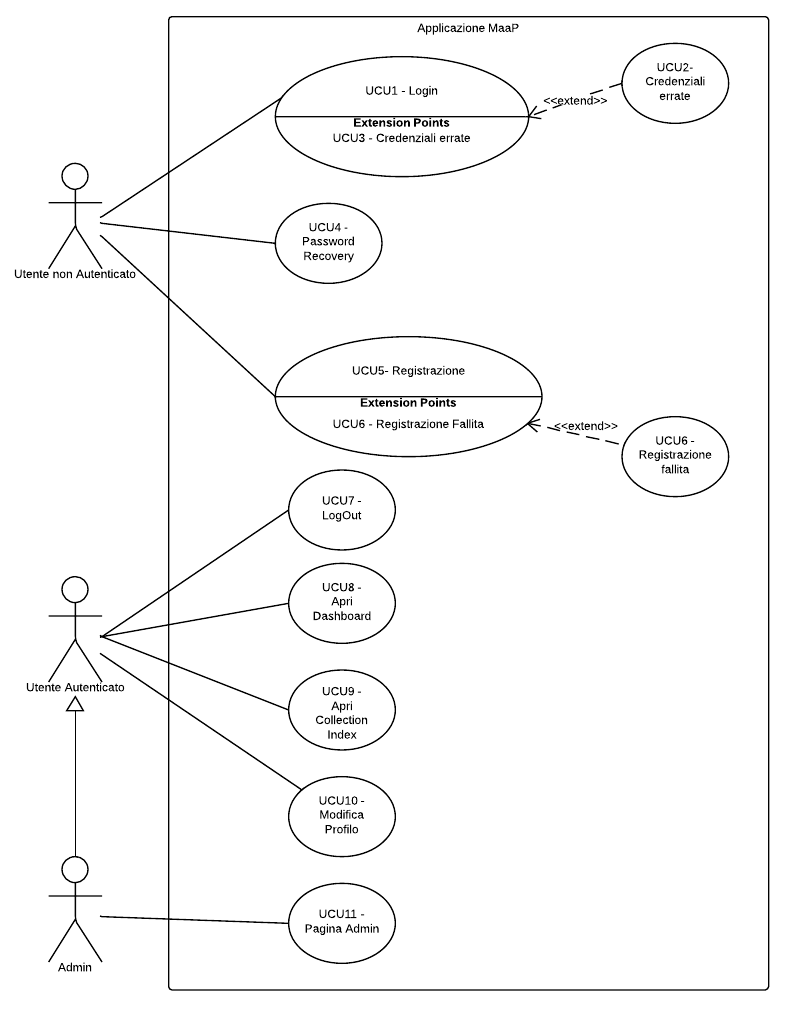
\includegraphics[width=12cm]{UML/UCU - Operazioni ad alto livello.png}
      \caption{UCU - Operazioni ad alto livello} 
    \end{figure}
      
    %Tabella 
      \begin{table}[h]
      \begin{longtabu}{  c | X  }
            
      \hline
      \multicolumn{2}{ | c | }{ \cellcolor[gray]{0.9} \textbf{UCU - Operazioni ad alto livello}} \\ 
      \hline
      
       & \\
      
      \textbf{Attori Primari} & Utente non autenticato, Utente autenticato, Admin \\ 
          \textbf{Attori Secondari} &   \\
          \textbf{Scopo e Descrizione} & L'Utente non autenticato può autenticarsi inserendo le credenziali nell'apposito form e  recuperare le stesse qualora le abbia perse.
L'Utente autenticato in qualsiasi punto dell'applicazione può accedere alle seguenti funzionalità: accedere alla Dashboard, effettuare il Logout , può scegliere una qualsiasi collection presente e può modificare i propri dati. 
L'Utente Admin eredita le funzionalità dell'Utente Autenticato ed in più accedere alla sezione "Admin" nella quale può creare o modificare un nuovo utente.  \\ 
          
          \textbf{Precondizioni}  & L'applicazione Maap è funzionante e pronta all'utilizzo.\\ 
          
          \textbf{Postcondizioni} & L'applicazione ha ricevuto le informazioni sulle operazioni che l'utente vuole eseguire. \\
          
          \textbf{Flusso Principale} & 1. Utente non autenticato esegue il login (UCU1); 
2. Utente non autenticato può recuperare la password (UCU4);
3. Utente non autenticato può richiedere la registrazione (UCU5);
4. L'utente autenticato può decidere di effettuare il logout (UCU7);
5. L'utente autenticato può visualizzare la Dashboard (UCU8);
6. L'utente autenticato può scegliere una collection e visualizzarla (UCU9);
7. L'utente autenticato può scegliere di modificare i propri dati (UCU10);
8. L'admin può accede alla sua pagina di amministrazione (UCU11).

 \\
           \textbf{Scenari Alternativi} & 1.1. L'utente visualizza un errore dato dall'inserimento errato delle credenziali. (UCU2);
2.1 L'utente visualizza un errore dato dal fallimento della registrazione (UCU6). \\
      \end{longtabu}
      \end{table}
\subsubsection{UCU1 - Login}
    
    \begin{figure}[H]
      %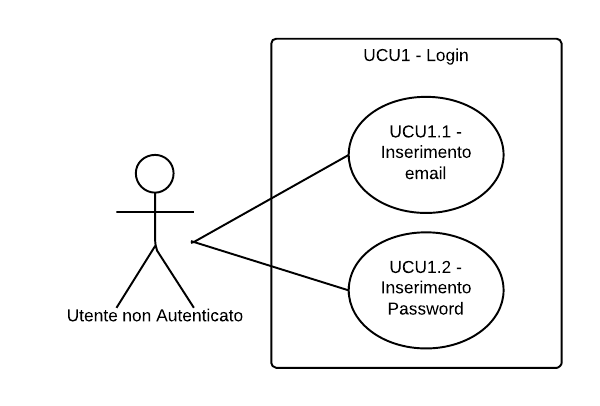
\includegraphics[width=12cm]{UML/UCU1 - Login.png}
      \caption{UCU - Operazioni ad alto livello} 
    \end{figure}
      
    %Tabella 
      \begin{table}[h]
      \begin{longtabu}{  c | X  }
            
      \hline
      \multicolumn{2}{ | c | }{ \cellcolor[gray]{0.9} \textbf{UCU1 - Login}} \\ 
      \hline
      
       & \\
      
      \textbf{Attori Primari} & Utente non autenticato  \\ 
          \textbf{Attori Secondari} &   \\
          \textbf{Scopo e Descrizione} & L'utente intende accedere all'applicazione, per farlo deve inserire le proprie credenziali composte da una email ed una password. \\ 
          
          \textbf{Precondizioni}  & L'applicazione è pronta a ricevere i dati e nel database è presente l'account dell'utente.\\ 
          
          \textbf{Postcondizioni} & L'utente è autenticato e rediretto alla pagina Dashboard. \\
          
          \textbf{Flusso Principale} & 1. L'utente inserisce l'email (UC1.1)
2. L'utente inserisce la password (UC1.2) \\
           \textbf{Scenari Alternativi} &  \\
      \end{longtabu}
      \end{table}
\subsubsection{UCU2 - Credenziali errate}
    
    \begin{figure}[H]
      %\includegraphics[width=12cm]{UML/UCU2 - Credenziali errate.png}
      \caption{UCU - Operazioni ad alto livello} 
    \end{figure}
      
    %Tabella 
      \begin{table}[h]
      \begin{longtabu}{  c | X  }
            
      \hline
      \multicolumn{2}{ | c | }{ \cellcolor[gray]{0.9} \textbf{UCU2 - Credenziali errate}} \\ 
      \hline
      
       & \\
      
      \textbf{Attori Primari} & Utente non autenticato  \\ 
          \textbf{Attori Secondari} &   \\
          \textbf{Scopo e Descrizione} & L'utente visualizza un messaggio di errore dato dall'inserimento di credenziali errate. \\ 
          
          \textbf{Precondizioni}  & L'applicazione ha verificato le credenziali inserite dall'utente.\\ 
          
          \textbf{Postcondizioni} & L'applicazione predispone la visualizzazione di un messaggio di errore. \\
          
          \textbf{Flusso Principale} &  \\
           \textbf{Scenari Alternativi} &  \\
      \end{longtabu}
      \end{table}
\subsubsection{UCU11.1.1 - Inserimento email}
    
    \begin{figure}[H]
      %\includegraphics[width=12cm]{UML/UCU11.1.1 - Inserimento email.png}
      \caption{UCU - Operazioni ad alto livello} 
    \end{figure}
      
    %Tabella 
      \begin{table}[h]
      \begin{longtabu}{  c | X  }
            
      \hline
      \multicolumn{2}{ | c | }{ \cellcolor[gray]{0.9} \textbf{UCU11.1.1 - Inserimento email}} \\ 
      \hline
      
       & \\
      
      \textbf{Attori Primari} & Admin \\ 
          \textbf{Attori Secondari} &   \\
          \textbf{Scopo e Descrizione} & L'admin può inserire in un campo di testo l'indirizzo email dell'utente da creare. \\ 
          
          \textbf{Precondizioni}  & Il sistema mette a disposizione dell'admin un campo di testo dove inserire la password del nuovo utente.\\ 
          
          \textbf{Postcondizioni} & Il campo di testo è stato compilato correttamente. \\
          
          \textbf{Flusso Principale} &  \\
           \textbf{Scenari Alternativi} &  \\
      \end{longtabu}
      \end{table}
\subsubsection{UCU11.1.3 - Definizione livello utente}
    
    \begin{figure}[H]
      %\includegraphics[width=12cm]{UML/UCU11.1.3 - Definizione livello utente.png}
      \caption{UCU - Operazioni ad alto livello} 
    \end{figure}
      
    %Tabella 
      \begin{table}[h]
      \begin{longtabu}{  c | X  }
            
      \hline
      \multicolumn{2}{ | c | }{ \cellcolor[gray]{0.9} \textbf{UCU11.1.3 - Definizione livello utente}} \\ 
      \hline
      
       & \\
      
      \textbf{Attori Primari} & Admin \\ 
          \textbf{Attori Secondari} &   \\
          \textbf{Scopo e Descrizione} & L'admin può selezionare il livello del nuovo utente, che potrà essere utente normale o admin. \\ 
          
          \textbf{Precondizioni}  & Il sistema mette a disposizione dell'admin un campo selezionabile dove poter definire il livello del nuovo utente.\\ 
          
          \textbf{Postcondizioni} & Il campo selezionabile è stato selezionato correttamente. \\
          
          \textbf{Flusso Principale} &  \\
           \textbf{Scenari Alternativi} &  \\
      \end{longtabu}
      \end{table}
\subsubsection{UCS1 - Creazione nuovo progetto}
    
    \begin{figure}[H]
      %\includegraphics[width=12cm]{UML/UCS1 - Creazione nuovo progetto.png}
      \caption{UCU - Operazioni ad alto livello} 
    \end{figure}
      
    %Tabella 
      \begin{table}[h]
      \begin{longtabu}{  c | X  }
            
      \hline
      \multicolumn{2}{ | c | }{ \cellcolor[gray]{0.9} \textbf{UCS1 - Creazione nuovo progetto}} \\ 
      \hline
      
       & \\
      
      \textbf{Attori Primari} & Sviluppatore \\ 
          \textbf{Attori Secondari} &   \\
          \textbf{Scopo e Descrizione} & Lo sviluppatore crea un nuovo progetto.
Alla creazione del nuovo progetto ne viene creato lo scheletro che si compone di:
- La creazione delle directory delle pagine web.
- La creazione del file di configurazione.
- L'inclusione delle librerie di sistema.
- La generazione del sistema di autenticazione che include la creazione del database delle credenziali e la generazione dell'utente admin di default. \\ 
          
          \textbf{Precondizioni}  & Il Framework è pronto a creare un nuovo progetto.\\ 
          
          \textbf{Postcondizioni} & Il Framework Maap ha creato un nuovo progetto completo di tutti i file necessari. \\
          
          \textbf{Flusso Principale} &  \\
           \textbf{Scenari Alternativi} &  \\
      \end{longtabu}
      \end{table}
\subsubsection{UCU11.3.1 - Eleva utente}
    
    \begin{figure}[H]
      %\includegraphics[width=12cm]{UML/UCU11.3.1 - Eleva utente.png}
      \caption{UCU - Operazioni ad alto livello} 
    \end{figure}
      
    %Tabella 
      \begin{table}[h]
      \begin{longtabu}{  c | X  }
            
      \hline
      \multicolumn{2}{ | c | }{ \cellcolor[gray]{0.9} \textbf{UCU11.3.1 - Eleva utente}} \\ 
      \hline
      
       & \\
      
      \textbf{Attori Primari} & Admin \\ 
          \textbf{Attori Secondari} &   \\
          \textbf{Scopo e Descrizione} & L'admin eleva l'utente selezionato a livello di admin. \\ 
          
          \textbf{Precondizioni}  & L'applicazione MaaP mette a disposizione dell'admin la pagina di modifica dell'utente selezionato.\\ 
          
          \textbf{Postcondizioni} & L'applicazione MaaP ha elevato l'utente selezionato dall'admin a livello di admin. \\
          
          \textbf{Flusso Principale} &  \\
           \textbf{Scenari Alternativi} &  \\
      \end{longtabu}
      \end{table}
\subsubsection{UCU11.3.2 - Declassa admin}
    
    \begin{figure}[H]
      %\includegraphics[width=12cm]{UML/UCU11.3.2 - Declassa admin.png}
      \caption{UCU - Operazioni ad alto livello} 
    \end{figure}
      
    %Tabella 
      \begin{table}[h]
      \begin{longtabu}{  c | X  }
            
      \hline
      \multicolumn{2}{ | c | }{ \cellcolor[gray]{0.9} \textbf{UCU11.3.2 - Declassa admin}} \\ 
      \hline
      
       & \\
      
      \textbf{Attori Primari} & Admin \\ 
          \textbf{Attori Secondari} &   \\
          \textbf{Scopo e Descrizione} & L'admin declassa l'admin selezionato al livello di utente normale. \\ 
          
          \textbf{Precondizioni}  & L'applicazione MaaP mette a disposizione dell'admin la pagina di modifica dell'utente selezionato.\\ 
          
          \textbf{Postcondizioni} & L'applicazione MaaP ha declassato l'utente selezionato dall'admin a livello di utente normale. \\
          
          \textbf{Flusso Principale} &  \\
           \textbf{Scenari Alternativi} &  \\
      \end{longtabu}
      \end{table}
\subsubsection{UCU11.3.3 - Modifica email utente}
    
    \begin{figure}[H]
      %\includegraphics[width=12cm]{UML/UCU11.3.3 - Modifica email utente.png}
      \caption{UCU - Operazioni ad alto livello} 
    \end{figure}
      
    %Tabella 
      \begin{table}[h]
      \begin{longtabu}{  c | X  }
            
      \hline
      \multicolumn{2}{ | c | }{ \cellcolor[gray]{0.9} \textbf{UCU11.3.3 - Modifica email utente}} \\ 
      \hline
      
       & \\
      
      \textbf{Attori Primari} & Admin \\ 
          \textbf{Attori Secondari} &   \\
          \textbf{Scopo e Descrizione} & L'admin modifica l'email dell'utente selezionato. \\ 
          
          \textbf{Precondizioni}  & L'applicazione MaaP mette a disposizione dell'admin la pagina di modifica dell'utente selezionato.\\ 
          
          \textbf{Postcondizioni} & L'applicazione MaaP ha modificato l'indirizzo email dell'utente selezionato dall'admin. \\
          
          \textbf{Flusso Principale} &  \\
           \textbf{Scenari Alternativi} &  \\
      \end{longtabu}
      \end{table}
\subsubsection{UCS - Operazioni ad alto livello}
    
    \begin{figure}[H]
      %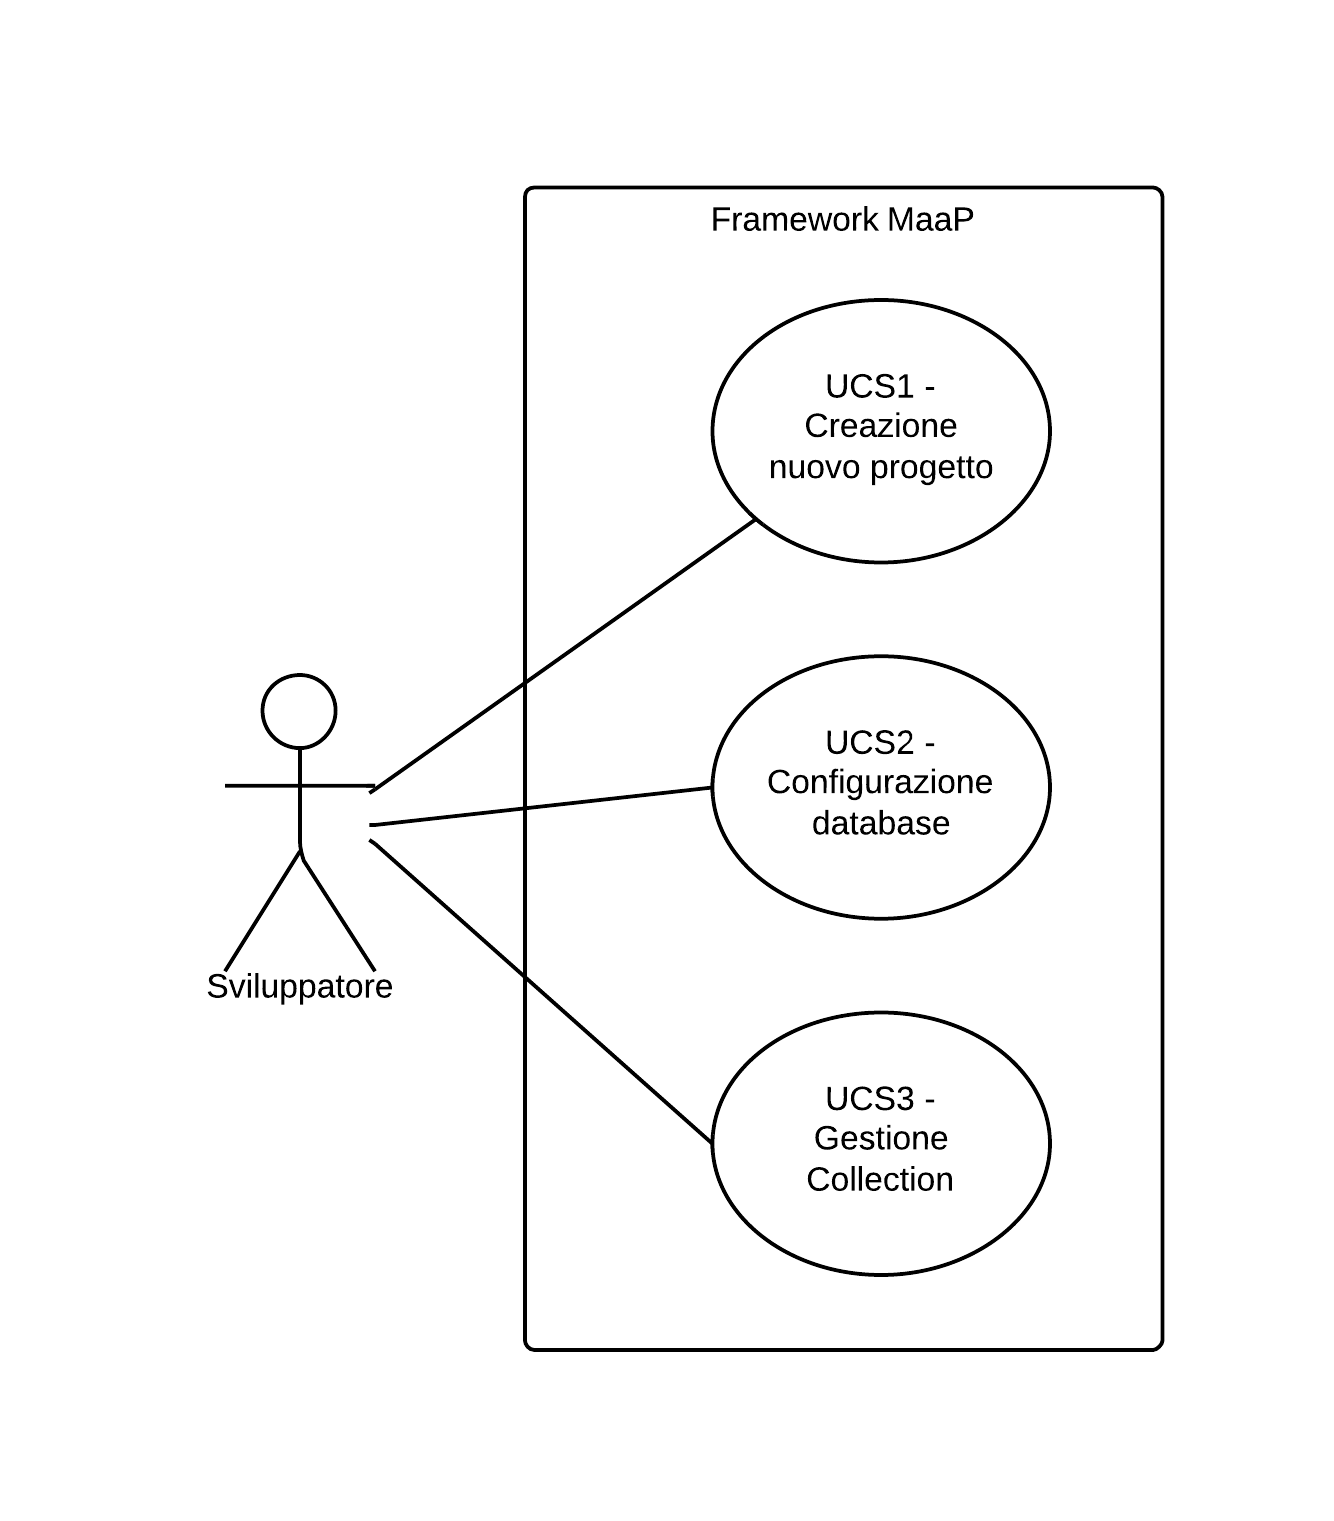
\includegraphics[width=12cm]{UML/UCS - Operazioni ad alto livello.png}
      \caption{UCU - Operazioni ad alto livello} 
    \end{figure}
      
    %Tabella 
      \begin{table}[h]
      \begin{longtabu}{  c | X  }
            
      \hline
      \multicolumn{2}{ | c | }{ \cellcolor[gray]{0.9} \textbf{UCS - Operazioni ad alto livello}} \\ 
      \hline
      
       & \\
      
      \textbf{Attori Primari} & Sviluppatore \\ 
          \textbf{Attori Secondari} &   \\
          \textbf{Scopo e Descrizione} & Lo sviluppatore avendo installato lo stack tecnologico richiesto per il funzionamento del Framework Maap può creare un nuovo progetto, dopo averlo creato potrà configurare i database e gestire le collection che desidera. \\ 
          
          \textbf{Precondizioni}  & Il Framework Maap è funzionante e pronto ad eseguire le azioni dello sviluppatore.\\ 
          
          \textbf{Postcondizioni} & Il Framework ha ottenuto le informazioni sulle azioni che l’utente desidera eseguire. \\
          
          \textbf{Flusso Principale} & 1. Lo Sviluppatore crea un nuovo progetto (UCS1);
2. Lo sviluppatore dopo aver creato il nuovo progetto può configurare i database (UCS2);
3. Lo sviluppatore con il nuovo progetto creato può gestire le collection che desidera generare (UCS3). \\
           \textbf{Scenari Alternativi} &  \\
      \end{longtabu}
      \end{table}
\subsubsection{UCU9.1.1 -  Apri show page attributi innestati}
    
    \begin{figure}[H]
      %\includegraphics[width=12cm]{UML/UCU9.1.1 -  Apri show page attributi innestati.png}
      \caption{UCU - Operazioni ad alto livello} 
    \end{figure}
      
    %Tabella 
      \begin{table}[h]
      \begin{longtabu}{  c | X  }
            
      \hline
      \multicolumn{2}{ | c | }{ \cellcolor[gray]{0.9} \textbf{UCU9.1.1 -  Apri show page attributi innestati}} \\ 
      \hline
      
       & \\
      
      \textbf{Attori Primari} & Utente autenticato, Admin \\ 
          \textbf{Attori Secondari} &   \\
          \textbf{Scopo e Descrizione} & L'utente può visualizzare gli attributi degli attributi innestati se presenti, del Document. \\ 
          
          \textbf{Precondizioni}  & L'applicazione riceve l'informazione necessaria per visualizzare l'attributo innestato selezionato dall'utente.\\ 
          
          \textbf{Postcondizioni} & L'applicazione visualizza gli attributi dell'attributo innestato. \\
          
          \textbf{Flusso Principale} &  \\
           \textbf{Scenari Alternativi} &  \\
      \end{longtabu}
      \end{table}
\subsubsection{UCU9.1.2 - Apri index page dell'array di Document}
    
    \begin{figure}[H]
      %\includegraphics[width=12cm]{UML/UCU9.1.2 - Apri index page dell'array di document.png}
      \caption{UCU - Operazioni ad alto livello} 
    \end{figure}
      
    %Tabella 
      \begin{table}[h]
      \begin{longtabu}{  c | X  }
            
      \hline
      \multicolumn{2}{ | c | }{ \cellcolor[gray]{0.9} \textbf{UCU9.1.2 - Apri index page dell'array di Document}} \\ 
      \hline
      
       & \\
      
      \textbf{Attori Primari} & Utente autenticato, Admin \\ 
          \textbf{Attori Secondari} &   \\
          \textbf{Scopo e Descrizione} & L'utente può visualizzare l'index page dell'array di Document. \\ 
          
          \textbf{Precondizioni}  & L'applicazione ha ricevuto la richiesta di visualizzazione dell'index page dell'array di Document dell'attributo selezionato dall'utente.\\ 
          
          \textbf{Postcondizioni} & L'applicazione mostra l'index page dell'array di Document. \\
          
          \textbf{Flusso Principale} &  \\
           \textbf{Scenari Alternativi} &  \\
      \end{longtabu}
      \end{table}
\subsubsection{UCU9.1.3 - Modifica Document}
    
    \begin{figure}[H]
      %\includegraphics[width=12cm]{UML/UCU9.1.3 - Modifica Document.png}
      \caption{UCU - Operazioni ad alto livello} 
    \end{figure}
      
    %Tabella 
      \begin{table}[h]
      \begin{longtabu}{  c | X  }
            
      \hline
      \multicolumn{2}{ | c | }{ \cellcolor[gray]{0.9} \textbf{UCU9.1.3 - Modifica Document}} \\ 
      \hline
      
       & \\
      
      \textbf{Attori Primari} & Admin \\ 
          \textbf{Attori Secondari} &   \\
          \textbf{Scopo e Descrizione} & L'Admin può modificare gli attributi del Document corrispondente alla page-show visualizzata. \\ 
          
          \textbf{Precondizioni}  & L'applicazione visualizza gli attributi del documento permettendo di modificarli.\\ 
          
          \textbf{Postcondizioni} & L'applicazione ha salvato le modifiche effettuate dall'admin al Document. \\
          
          \textbf{Flusso Principale} &  \\
           \textbf{Scenari Alternativi} & 1. L'admin annulla le modifiche al Document. \\
      \end{longtabu}
      \end{table}
\subsubsection{UCU9.1.4 - Elimina Document}
    
    \begin{figure}[H]
      %\includegraphics[width=12cm]{UML/UCU9.1.4 - Elimina Document.png}
      \caption{UCU - Operazioni ad alto livello} 
    \end{figure}
      
    %Tabella 
      \begin{table}[h]
      \begin{longtabu}{  c | X  }
            
      \hline
      \multicolumn{2}{ | c | }{ \cellcolor[gray]{0.9} \textbf{UCU9.1.4 - Elimina Document}} \\ 
      \hline
      
       & \\
      
      \textbf{Attori Primari} & Admin \\ 
          \textbf{Attori Secondari} &   \\
          \textbf{Scopo e Descrizione} & L'admin può eliminare il Document corrispondente alla show-page visualizzata. \\ 
          
          \textbf{Precondizioni}  & L'applicazione permette l'eliminazione del Document.\\ 
          
          \textbf{Postcondizioni} & L'applicazione ha eliminato il Document dalla collection. \\
          
          \textbf{Flusso Principale} &  \\
           \textbf{Scenari Alternativi} &  \\
      \end{longtabu}
      \end{table}
\subsubsection{UCU9.2 - Filtra risultati}
    
    \begin{figure}[H]
      %\includegraphics[width=12cm]{UML/UCU9.2 - Filtra risultati.png}
      \caption{UCU - Operazioni ad alto livello} 
    \end{figure}
      
    %Tabella 
      \begin{table}[h]
      \begin{longtabu}{  c | X  }
            
      \hline
      \multicolumn{2}{ | c | }{ \cellcolor[gray]{0.9} \textbf{UCU9.2 - Filtra risultati}} \\ 
      \hline
      
       & \\
      
      \textbf{Attori Primari} & Utente autenticato, Admin \\ 
          \textbf{Attori Secondari} &   \\
          \textbf{Scopo e Descrizione} & L'utente può filtrare i documenti mostrati dalla collection-index. \\ 
          
          \textbf{Precondizioni}  & L'applicazione, nella pagina visualizzata, mette a disposizione filtri.\\ 
          
          \textbf{Postcondizioni} & L'applicazione ha filtrato i documenti visualizzati secondo i filtri richiesti dall'utente. \\
          
          \textbf{Flusso Principale} &  \\
           \textbf{Scenari Alternativi} &  \\
      \end{longtabu}
      \end{table}
\subsubsection{UCU9.3 - Esegui azione personalizzata}
    
    \begin{figure}[H]
      %\includegraphics[width=12cm]{UML/UCU9.3 - Esegui azione personalizzata.png}
      \caption{UCU - Operazioni ad alto livello} 
    \end{figure}
      
    %Tabella 
      \begin{table}[h]
      \begin{longtabu}{  c | X  }
            
      \hline
      \multicolumn{2}{ | c | }{ \cellcolor[gray]{0.9} \textbf{UCU9.3 - Esegui azione personalizzata}} \\ 
      \hline
      
       & \\
      
      \textbf{Attori Primari} & Utente autenticato, Admin \\ 
          \textbf{Attori Secondari} &   \\
          \textbf{Scopo e Descrizione} & L'utente può eseguire operazioni personalizzate tramite uso di bottoni se predisposti nella pagina visualizzata. \\ 
          
          \textbf{Precondizioni}  & L'applicazione  nella pagina visualizzata ha bottoni predisposti per l'esecuzione di azioni personalizzate.\\ 
          
          \textbf{Postcondizioni} & L'applicazione a seconda dell'azione eseguita dall'utente ha svolto le sue funzioni. \\
          
          \textbf{Flusso Principale} &  \\
           \textbf{Scenari Alternativi} &  \\
      \end{longtabu}
      \end{table}
\subsubsection{UCU9.5 - Elimina Document}
    
    \begin{figure}[H]
      %\includegraphics[width=12cm]{UML/UCU9.5 - Elimina Document.png}
      \caption{UCU - Operazioni ad alto livello} 
    \end{figure}
      
    %Tabella 
      \begin{table}[h]
      \begin{longtabu}{  c | X  }
            
      \hline
      \multicolumn{2}{ | c | }{ \cellcolor[gray]{0.9} \textbf{UCU9.5 - Elimina Document}} \\ 
      \hline
      
       & \\
      
      \textbf{Attori Primari} & Admin \\ 
          \textbf{Attori Secondari} &   \\
          \textbf{Scopo e Descrizione} & L'admin può eliminare un Document direttamente dalla pagina collection index visualizzata. \\ 
          
          \textbf{Precondizioni}  & L'applicazione ha predisposto per ogni Document visualizzato nella collection, la possibilità di eliminarlo.\\ 
          
          \textbf{Postcondizioni} & L'applicazione ha eliminato il Document selezionato dalla collection. \\
          
          \textbf{Flusso Principale} &  \\
           \textbf{Scenari Alternativi} &  \\
      \end{longtabu}
      \end{table}
\subsubsection{UCU9.1 - Apri show-page Document}
    
    \begin{figure}[H]
      %\includegraphics[width=12cm]{UML/UCU9.1 - Apri show-page Document.png}
      \caption{UCU - Operazioni ad alto livello} 
    \end{figure}
      
    %Tabella 
      \begin{table}[h]
      \begin{longtabu}{  c | X  }
            
      \hline
      \multicolumn{2}{ | c | }{ \cellcolor[gray]{0.9} \textbf{UCU9.1 - Apri show-page Document}} \\ 
      \hline
      
       & \\
      
      \textbf{Attori Primari} & Utente autenticato, Admin \\ 
          \textbf{Attori Secondari} &   \\
          \textbf{Scopo e Descrizione} & L'utente visualizza la pagina show-page corrispondente ad un Document selezionato visualizzandone gli attributi in forma tabellare.
In questa pagina può aprire la show page o l'index page dell'array di Document degli attributi innestati se presenti, eseguire un'operazione personalizzata se ne sono disponibili.
L'admin può eliminare il Document a cui la show page corrisponde o modificarlo. \\ 
          
          \textbf{Precondizioni}  & L'applicazione ha ottenuto l'informazione necessaria per poter visualizzare la show-page correlata al Document selezionato dall'utente.\\ 
          
          \textbf{Postcondizioni} & L'applicazione mostra all'utente la show-page corrispondente ed è pronta ad eseguire azioni. \\
          
          \textbf{Flusso Principale} & 1. L'utente autenticato può aprire la show page degli attributi innestati. (UCU9.1.1);
2. L'utente autenticato può aprire l'index page dell'array di Document (UCU9.1.2);
3. L'utente autenticato può eseguire se presente un'operazione personalizzata (UCU9.3);
4. L'admin può modificare il Document (UCU9.1.3);
5. L'admin può eliminare il Document (UCU9.1.4). \\
           \textbf{Scenari Alternativi} &  \\
      \end{longtabu}
      \end{table}
\subsubsection{UCU9.4 - Modifica Document}
    
    \begin{figure}[H]
      %\includegraphics[width=12cm]{UML/UCU9.4 - Modifica Document.png}
      \caption{UCU - Operazioni ad alto livello} 
    \end{figure}
      
    %Tabella 
      \begin{table}[h]
      \begin{longtabu}{  c | X  }
            
      \hline
      \multicolumn{2}{ | c | }{ \cellcolor[gray]{0.9} \textbf{UCU9.4 - Modifica Document}} \\ 
      \hline
      
       & \\
      
      \textbf{Attori Primari} & Admin \\ 
          \textbf{Attori Secondari} &   \\
          \textbf{Scopo e Descrizione} & L'admin può selezionare un Document per andarlo a modificare. \\ 
          
          \textbf{Precondizioni}  & L'applicazione mostra in forma tabellare tutti i Document della collection predisponendo la possibilità per ognuno di modifica.\\ 
          
          \textbf{Postcondizioni} & L'applicazione ha salvato le modifiche apportate dall'utente al Document. \\
          
          \textbf{Flusso Principale} &  \\
           \textbf{Scenari Alternativi} & 1. L'admin non ha modificato il Document. \\
      \end{longtabu}
      \end{table}
\subsubsection{UCU11.1 - Creazione utente}
    
    \begin{figure}[H]
      %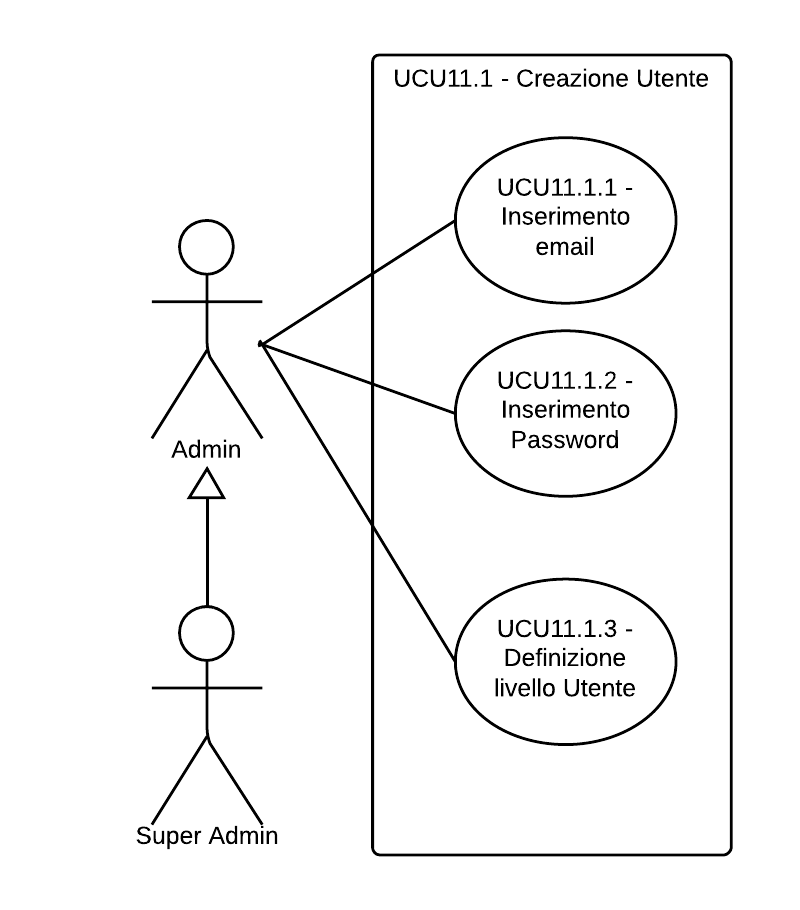
\includegraphics[width=12cm]{UML/UCU11.1 - Creazione utente.png}
      \caption{UCU - Operazioni ad alto livello} 
    \end{figure}
      
    %Tabella 
      \begin{table}[h]
      \begin{longtabu}{  c | X  }
            
      \hline
      \multicolumn{2}{ | c | }{ \cellcolor[gray]{0.9} \textbf{UCU11.1 - Creazione utente}} \\ 
      \hline
      
       & \\
      
      \textbf{Attori Primari} & Admin \\ 
          \textbf{Attori Secondari} &   \\
          \textbf{Scopo e Descrizione} & L'admin entra in un'apposita pagina di creazione utente, dalla quale inserisce i dati e crea un nuovo utente nel database. \\ 
          
          \textbf{Precondizioni}  & Il sistema ha reindirizzato l'admin nella pagina di creazione di un nuovo utente.\\ 
          
          \textbf{Postcondizioni} & Il sistema ha creato un nuovo utente nel database con i dati immessi dall'admin. \\
          
          \textbf{Flusso Principale} & 1. L'admin inserisce l'indirizzo email del nuovo utente (UCU11.1.1);
2. L'admin inserisce la password del nuovo utente (UCU11.1.2); 
3. L'admin definisce il livello del nuovo utente (UCU11.1.3). \\
           \textbf{Scenari Alternativi} & 1. L'admin lascia la pagina senza aver salvato le modifiche;
2. I dati inseriti dall'admin non sono corretti e fallisce la registrazione. \\
      \end{longtabu}
      \end{table}
\subsubsection{UCU11.3 - Apri show-page Utente}
    
    \begin{figure}[H]
      %\includegraphics[width=12cm]{UML/UCU11.3 - Apri show-page Utente.png}
      \caption{UCU - Operazioni ad alto livello} 
    \end{figure}
      
    %Tabella 
      \begin{table}[h]
      \begin{longtabu}{  c | X  }
            
      \hline
      \multicolumn{2}{ | c | }{ \cellcolor[gray]{0.9} \textbf{UCU11.3 - Apri show-page Utente}} \\ 
      \hline
      
       & \\
      
      \textbf{Attori Primari} & Admin \\ 
          \textbf{Attori Secondari} &   \\
          \textbf{Scopo e Descrizione} & L'admin visualizza la tabella degli utenti registrati e può aprire la relativa show-page di uno di essi tramite link. \\ 
          
          \textbf{Precondizioni}  & L'applicazione mette a disposizione dell'admin la visualizzazione della show-index dell'utente.\\ 
          
          \textbf{Postcondizioni} & L'applicazione MaaP ha reindirizzato l'admin nella Collection-show dell'utente selezionato. \\
          
          \textbf{Flusso Principale} & 1. L'admin può elevare un utente normale a livello di admin (UCU11.3.1);
2. L'admin può declassare un admin a livello di utente normale (UCU11.3.2);
3. L'admin può modificare l'email dell'utente selezionato (UCU11.3.3);
4. L'admin può modificare la password dell'utente selezionato (UCU11.3.4); \\
           \textbf{Scenari Alternativi} &  \\
      \end{longtabu}
      \end{table}
\subsubsection{UCU11.3.4 - Modifica Password Utente}
    
    \begin{figure}[H]
      %\includegraphics[width=12cm]{UML/UCU11.3.4 - Modifica Password Utente.png}
      \caption{UCU - Operazioni ad alto livello} 
    \end{figure}
      
    %Tabella 
      \begin{table}[h]
      \begin{longtabu}{  c | X  }
            
      \hline
      \multicolumn{2}{ | c | }{ \cellcolor[gray]{0.9} \textbf{UCU11.3.4 - Modifica Password Utente}} \\ 
      \hline
      
       & \\
      
      \textbf{Attori Primari} & Admin \\ 
          \textbf{Attori Secondari} &   \\
          \textbf{Scopo e Descrizione} & L'admin può modificare la password dell'utente corrispondente alla show-page visualizzata. \\ 
          
          \textbf{Precondizioni}  & L'applicazione MaaP mette a disposizione dell'admin la pagina di modifica dell'utente selezionato.\\ 
          
          \textbf{Postcondizioni} & L'applicazione ha modificato la password dell'utente relativo alla show-page corrispondente. \\
          
          \textbf{Flusso Principale} &  \\
           \textbf{Scenari Alternativi} &  \\
      \end{longtabu}
      \end{table}
\subsubsection{UCS3 - Gestione Collection}
    
    \begin{figure}[H]
      %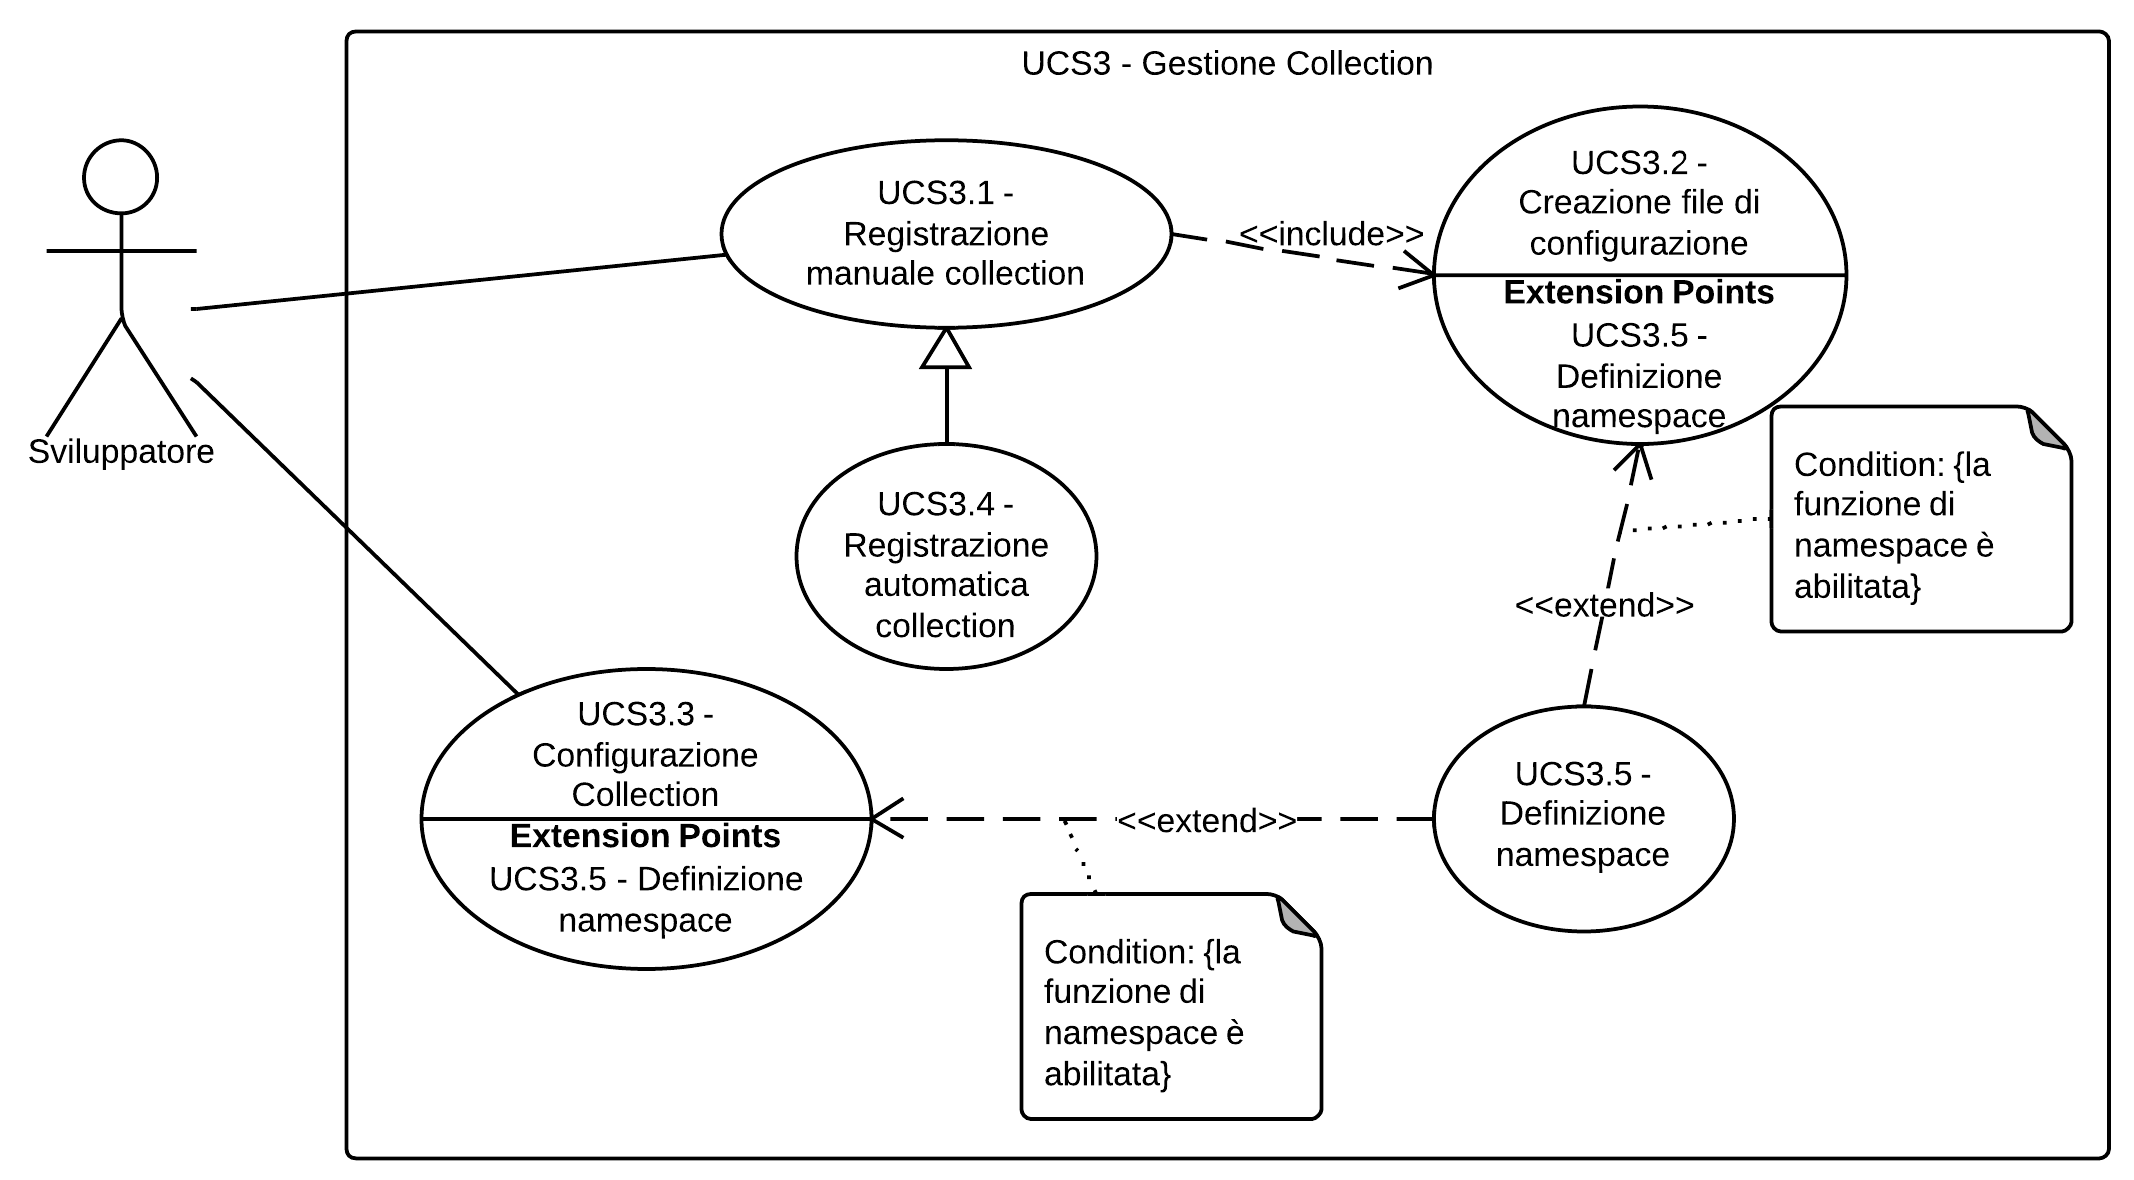
\includegraphics[width=12cm]{UML/UCS3 - Gestione Collection.png}
      \caption{UCU - Operazioni ad alto livello} 
    \end{figure}
      
    %Tabella 
      \begin{table}[h]
      \begin{longtabu}{  c | X  }
            
      \hline
      \multicolumn{2}{ | c | }{ \cellcolor[gray]{0.9} \textbf{UCS3 - Gestione Collection}} \\ 
      \hline
      
       & \\
      
      \textbf{Attori Primari} & Sviluppatore \\ 
          \textbf{Attori Secondari} &   \\
          \textbf{Scopo e Descrizione} & Lo sviluppatore, con il progetto creato, può registrare manualmente una collection o usufruire della registrazione automatica, con relativa creazione del file di configurazione della stessa.
Può poi configurare le collection create. \\ 
          
          \textbf{Precondizioni}  & Il Framework MaaP è pronto, il progetto è stato creato e lo sviluppatore intende gestire le collection.\\ 
          
          \textbf{Postcondizioni} & Il Framework ha le informazioni per eseguire le azioni richieste dallo sviluppatore. \\
          
          \textbf{Flusso Principale} & Il Framework ha appreso le informazioni necessarie sulle azioni che lo sviluppatore vuole eseguire. \\
           \textbf{Scenari Alternativi} &  \\
      \end{longtabu}
      \end{table}
\subsubsection{UCS3.1 - Registrazione manuale Collection}
    
    \begin{figure}[H]
      %\includegraphics[width=12cm]{UML/UCS3.1 - Registrazione manuale Collection.png}
      \caption{UCU - Operazioni ad alto livello} 
    \end{figure}
      
    %Tabella 
      \begin{table}[h]
      \begin{longtabu}{  c | X  }
            
      \hline
      \multicolumn{2}{ | c | }{ \cellcolor[gray]{0.9} \textbf{UCS3.1 - Registrazione manuale Collection}} \\ 
      \hline
      
       & \\
      
      \textbf{Attori Primari} & Sviluppatore \\ 
          \textbf{Attori Secondari} &   \\
          \textbf{Scopo e Descrizione} & Lo sviluppatore registra manualmente una Collection creando tutti i file necessari al suo funzionamento. \\ 
          
          \textbf{Precondizioni}  & Il Framework MaaP è funzionante e lo sviluppatore ha creato un progetto.\\ 
          
          \textbf{Postcondizioni} & Il Framework MaaP ha registrato correttamente la nuova Collection. \\
          
          \textbf{Flusso Principale} &  \\
           \textbf{Scenari Alternativi} &  \\
      \end{longtabu}
      \end{table}
\subsubsection{UCS3.2 - Creazione file di configurazione}
    
    \begin{figure}[H]
      %\includegraphics[width=12cm]{UML/UCS3.2 - Creazione file di configurazione.png}
      \caption{UCU - Operazioni ad alto livello} 
    \end{figure}
      
    %Tabella 
      \begin{table}[h]
      \begin{longtabu}{  c | X  }
            
      \hline
      \multicolumn{2}{ | c | }{ \cellcolor[gray]{0.9} \textbf{UCS3.2 - Creazione file di configurazione}} \\ 
      \hline
      
       & \\
      
      \textbf{Attori Primari} & Sviluppatore \\ 
          \textbf{Attori Secondari} &   \\
          \textbf{Scopo e Descrizione} & Nella registrazione di una nuova Collection deve essere creato un file di configurazione per essa. \\ 
          
          \textbf{Precondizioni}  & Il Framework MaaP sta registrando una nuova Collection.\\ 
          
          \textbf{Postcondizioni} & Il Framework MaaP ha creato il file di configurazione per la nuova Collection. \\
          
          \textbf{Flusso Principale} &  \\
           \textbf{Scenari Alternativi} &  \\
      \end{longtabu}
      \end{table}
\subsubsection{UCS3.4 - Registrazione automatica Collection}
    
    \begin{figure}[H]
      %\includegraphics[width=12cm]{UML/UCS3.4 - Registrazione automatica Collection.png}
      \caption{UCU - Operazioni ad alto livello} 
    \end{figure}
      
    %Tabella 
      \begin{table}[h]
      \begin{longtabu}{  c | X  }
            
      \hline
      \multicolumn{2}{ | c | }{ \cellcolor[gray]{0.9} \textbf{UCS3.4 - Registrazione automatica Collection}} \\ 
      \hline
      
       & \\
      
      \textbf{Attori Primari} & Sviluppatore \\ 
          \textbf{Attori Secondari} &   \\
          \textbf{Scopo e Descrizione} & Lo sviluppatore crea automaticamente una nuova Collection da linea di comando. \\ 
          
          \textbf{Precondizioni}  & Il Framework MaaP è funzionante e lo sviluppatore ha creato un progetto.\\ 
          
          \textbf{Postcondizioni} & Il Framework MaaP ha registrato correttamente la nuova Collection. \\
          
          \textbf{Flusso Principale} &  \\
           \textbf{Scenari Alternativi} &  \\
      \end{longtabu}
      \end{table}
\subsubsection{UCS3.3 - Configurazione Collection}
    
    \begin{figure}[H]
      %\includegraphics[width=12cm]{UML/UCS3.3 - Configurazione Collection.png}
      \caption{UCU - Operazioni ad alto livello} 
    \end{figure}
      
    %Tabella 
      \begin{table}[h]
      \begin{longtabu}{  c | X  }
            
      \hline
      \multicolumn{2}{ | c | }{ \cellcolor[gray]{0.9} \textbf{UCS3.3 - Configurazione Collection}} \\ 
      \hline
      
       & \\
      
      \textbf{Attori Primari} & Sviluppatore \\ 
          \textbf{Attori Secondari} &   \\
          \textbf{Scopo e Descrizione} & Lo sviluppatore modifica il file di configurazione di una Collection creata. \\ 
          
          \textbf{Precondizioni}  & Il Framework MaaP ha registrato correttamente la Collection da configurare.\\ 
          
          \textbf{Postcondizioni} & Il Framework MaaP ha configurato correttamente la Collection modificata dallo sviluppatore. \\
          
          \textbf{Flusso Principale} & 1. Lo sviluppatore personalizza la index page della Collection (UCS3.3.1);
2. Lo sviluppatore personalizza la show page della Collection (UCS3.3.2);
3. Lo sviluppatore rinomina il titolo della Collection che verrà visualizzato nel menu di navigazione (UCS3.3.3);
4. Lo sviluppatore definisce l'ordine di visualizzazione della Collection nel menu di navigazione (UCS3.3.4); \\
           \textbf{Scenari Alternativi} &  \\
      \end{longtabu}
      \end{table}
\subsubsection{UCS3.3.1 - Personalizzazione index page}
    
    \begin{figure}[H]
      %\includegraphics[width=12cm]{UML/UCS3.3.1 - Personalizzazione index page.png}
      \caption{UCU - Operazioni ad alto livello} 
    \end{figure}
      
    %Tabella 
      \begin{table}[h]
      \begin{longtabu}{  c | X  }
            
      \hline
      \multicolumn{2}{ | c | }{ \cellcolor[gray]{0.9} \textbf{UCS3.3.1 - Personalizzazione index page}} \\ 
      \hline
      
       & \\
      
      \textbf{Attori Primari} & Sviluppatore \\ 
          \textbf{Attori Secondari} &   \\
          \textbf{Scopo e Descrizione} & Lo sviluppatore personalizza la index page della Collection selezionata. \\ 
          
          \textbf{Precondizioni}  & Il Framework MaaP è funzionante e la Collection da configurare è stata registrata.\\ 
          
          \textbf{Postcondizioni} & Il Framework MaaP ha configurato correttamente la index page della Collection. \\
          
          \textbf{Flusso Principale} & 1. Lo sviluppatore definisce gli attributi da visualizzare (UCS3.3.1.1);
2. Lo sviluppatore definisce l'ordinamento degli attributi (UCS3.3.1.2);
3. Lo sviluppatore definisce il limite degli elementi da visualizzare (UCS3.3.1.3);
4. Lo sviluppatore definisce quale attributo è selezionabile (UCS3.3.1.4);
5. Lo sviluppatore definisce una query che visualizzerà un sottoinsieme di Document dalla Collection (UCS3.3.1.5);
6. Lo sviluppatore definisce come attributo un attributo innestato o un array di attributi (UCS3.3u.1.6);
7. Lo sviluppatore personalizza la tipologia di filtri da visualizzare (UCS3.3.1.7);
8. Lo sviluppatore definisce delle trasformazioni sugli attributi (UCS3.3.1.8);
9. Lo sviluppatore definisce delle azioni personalizzate (UCS3.3.1.9). \\
           \textbf{Scenari Alternativi} &  \\
      \end{longtabu}
      \end{table}
\subsubsection{UCS3.3.1.1 - Definizione attributi da visualizzare}
    
    \begin{figure}[H]
      %\includegraphics[width=12cm]{UML/UCS3.3.1.1 - Definizione attributi da visualizzare.png}
      \caption{UCU - Operazioni ad alto livello} 
    \end{figure}
      
    %Tabella 
      \begin{table}[h]
      \begin{longtabu}{  c | X  }
            
      \hline
      \multicolumn{2}{ | c | }{ \cellcolor[gray]{0.9} \textbf{UCS3.3.1.1 - Definizione attributi da visualizzare}} \\ 
      \hline
      
       & \\
      
      \textbf{Attori Primari} & Sviluppatore \\ 
          \textbf{Attori Secondari} &   \\
          \textbf{Scopo e Descrizione} & Lo sviluppatore all'interno del file di configurazione della Collection specifica quali attributi visualizzare nella index page. \\ 
          
          \textbf{Precondizioni}  & Il Framework MaaP è funzionante e la Collection è registrata.\\ 
          
          \textbf{Postcondizioni} & Il Framework MaaP ha apportato le modifiche alla configurazione della Collection. \\
          
          \textbf{Flusso Principale} &  \\
           \textbf{Scenari Alternativi} &  \\
      \end{longtabu}
      \end{table}
\subsubsection{UCS3.3.1.2 - Definizione ordinamento attributi}
    
    \begin{figure}[H]
      %\includegraphics[width=12cm]{UML/UCS3.3.1.2 - Definizione ordinamento attributi.png}
      \caption{UCU - Operazioni ad alto livello} 
    \end{figure}
      
    %Tabella 
      \begin{table}[h]
      \begin{longtabu}{  c | X  }
            
      \hline
      \multicolumn{2}{ | c | }{ \cellcolor[gray]{0.9} \textbf{UCS3.3.1.2 - Definizione ordinamento attributi}} \\ 
      \hline
      
       & \\
      
      \textbf{Attori Primari} & Sviluppatore \\ 
          \textbf{Attori Secondari} &   \\
          \textbf{Scopo e Descrizione} & Lo sviluppatore all'interno del file di configurazione della Collection definisce un ordinamento di default e specifica quali attributi sono ordinabili o no. \\ 
          
          \textbf{Precondizioni}  & Il Framework MaaP è funzionante e la Collection è registrata.\\ 
          
          \textbf{Postcondizioni} & Il Framework MaaP ha apportato le modifiche alla configurazione della Collection. \\
          
          \textbf{Flusso Principale} &  \\
           \textbf{Scenari Alternativi} &  \\
      \end{longtabu}
      \end{table}
\subsubsection{UCS3.3.1.3 - Definizione limite elementi da visualizzare}
    
    \begin{figure}[H]
      %\includegraphics[width=12cm]{UML/UCS3.3.1.3 - Definizione limite elementi da visualizzare.png}
      \caption{UCU - Operazioni ad alto livello} 
    \end{figure}
      
    %Tabella 
      \begin{table}[h]
      \begin{longtabu}{  c | X  }
            
      \hline
      \multicolumn{2}{ | c | }{ \cellcolor[gray]{0.9} \textbf{UCS3.3.1.3 - Definizione limite elementi da visualizzare}} \\ 
      \hline
      
       & \\
      
      \textbf{Attori Primari} & Sviluppatore \\ 
          \textbf{Attori Secondari} &   \\
          \textbf{Scopo e Descrizione} & Lo sviluppatore all'interno del file di configurazione della Collection specifica quanti Document per pagina verranno visualizzati nella index page. \\ 
          
          \textbf{Precondizioni}  & Il Framework MaaP è funzionante e la Collection è registrata.\\ 
          
          \textbf{Postcondizioni} & Il Framework MaaP ha apportato le modifiche alla configurazione della Collection. \\
          
          \textbf{Flusso Principale} &  \\
           \textbf{Scenari Alternativi} &  \\
      \end{longtabu}
      \end{table}
\subsubsection{UCS3.3.1.4 - Definizione attributo selezionabile}
    
    \begin{figure}[H]
      %\includegraphics[width=12cm]{UML/UCS3.3.1.4 - Definizione attributo selezionabile.png}
      \caption{UCU - Operazioni ad alto livello} 
    \end{figure}
      
    %Tabella 
      \begin{table}[h]
      \begin{longtabu}{  c | X  }
            
      \hline
      \multicolumn{2}{ | c | }{ \cellcolor[gray]{0.9} \textbf{UCS3.3.1.4 - Definizione attributo selezionabile}} \\ 
      \hline
      
       & \\
      
      \textbf{Attori Primari} & Sviluppatore \\ 
          \textbf{Attori Secondari} &   \\
          \textbf{Scopo e Descrizione} & Lo sviluppatore all'interno del file di configurazione della Collection specifica quale attributo sarà identificato come chiave per poter accedere alla show page del corrispondente Document. \\ 
          
          \textbf{Precondizioni}  & Il Framework MaaP è funzionante e la Collection è registrata.\\ 
          
          \textbf{Postcondizioni} & Il Framework MaaP ha apportato le modifiche alla configurazione della Collection. \\
          
          \textbf{Flusso Principale} &  \\
           \textbf{Scenari Alternativi} &  \\
      \end{longtabu}
      \end{table}
\subsubsection{UCS3.3.1.5 - Definizione della index-query}
    
    \begin{figure}[H]
      %\includegraphics[width=12cm]{UML/UCS3.3.1.5 - Definizione della index-query.png}
      \caption{UCU - Operazioni ad alto livello} 
    \end{figure}
      
    %Tabella 
      \begin{table}[h]
      \begin{longtabu}{  c | X  }
            
      \hline
      \multicolumn{2}{ | c | }{ \cellcolor[gray]{0.9} \textbf{UCS3.3.1.5 - Definizione della index-query}} \\ 
      \hline
      
       & \\
      
      \textbf{Attori Primari} & Sviluppatore \\ 
          \textbf{Attori Secondari} &   \\
          \textbf{Scopo e Descrizione} & Lo sviluppatore all'interno del file di configurazione della Collection definisce delle query che andranno a selezionare un sottoinsieme di Document dalla Collection. \\ 
          
          \textbf{Precondizioni}  & Il Framework MaaP è funzionante e la Collection è registrata.\\ 
          
          \textbf{Postcondizioni} & Il Framework MaaP ha apportato le modifiche alla configurazione della Collection. \\
          
          \textbf{Flusso Principale} &  \\
           \textbf{Scenari Alternativi} &  \\
      \end{longtabu}
      \end{table}